\documentclass[a4paper,12pt]{report}
\usepackage{graphicx}
\usepackage{cancel}	%para cancelar expresiones en fórmulas
\usepackage{multicol}
\usepackage{multirow}
\usepackage{amsmath}
\usepackage{float}
\usepackage{url}
\usepackage{color}
\usepackage{tablefootnote}
\usepackage[12pt]{moresize}	%más tamaños de letra
\usepackage{bm}	%bold para math

\usepackage{titlesec}
%\titleformat{\chapter}[display]
%{\normalfont\bfseries}{}{12pt}{\Huge}	%quitar header de chapter

\usepackage{siunitx}	%support for units, numbers
\sisetup{output-decimal-marker={.}, separate-uncertainty}

\usepackage{hyperref}
\hypersetup{
	colorlinks=true,
	linkcolor=blue,
	citecolor=red,
	bookmarksopen=true,
	bookmarksopenlevel=1,
	urlcolor=blue
}

\usepackage{tikz}	%%TIKZ for drawings, shapes
\usetikzlibrary{positioning}
\tikzset{
	nodo/.style={
		rectangle,
		draw,
		black,
		thick,
		rounded corners,
		node distance=1.5cm,
		inner sep=0.3cm,
		font=\large
	}
}

%%% NOMBRES DE COSAS
\renewcommand{\abstractname}{Abstract}
\renewcommand{\figurename}{Figure}
\renewcommand{\tablename}{Table}
\renewcommand{\contentsname}{Table of Contents}
\renewcommand{\appendixname}{Appendix}
\renewcommand{\bibname}{References}
\renewcommand{\chaptername}{Part}

%%% COMANDOS COMUNES
\newcommand{\dif}{\text{d}}
\newcommand{\ddt}[1]{\frac{\dif #1}{\dif t}}
\newcommand{\der}[2]{\frac{\dif #1}{\dif #2}}
\newcommand{\mder}[3]{\frac{\dif^{#3}#1}{\dif #2^{#3}}}		%derivada múltiple
\newcommand{\norm}[1]{\left\| #1 \right\|}
\newcommand{\an}{($\alpha$,n) }
\newcommand{\Aliso}{\textsuperscript{27}Al }
\newcommand{\Piso}{\textsuperscript{30}P }
\newcommand{\Na}{\textsuperscript{22}Na }

%%%%%%%%%%%%%%%%%%%%%%%%%%%%%%%%%%%%%%%%%%%%%%%%%%%%%%%%%
\usepackage[a4paper]{geometry}
\geometry{top=2cm,bottom=2cm,left=1.8cm,right=1.8cm}
\usepackage{setspace}	%interlineado
\onehalfspace	%interlineado 1.5

\makeindex
%%%%%%%%%%%%%%%%%%%%%%%%%%%%%%%%%%%%%%%%%%%%%%%%%%%%%%%%%
\begin{document}
\begin{titlepage}
	\centering
	\Large Master's Thesis\par
	\Huge Inter-University Master's degree in Nuclear Physics\par
	\vspace*{3cm}
	\HUGE \textbf{Measurements of ($\bm{\alpha}$,n) reactions in CNA/HiSPANoS}\par	%TBD? más largo?
	\vspace{1cm}
	
\includegraphics[width=0.35\textwidth]{us.png}\\
	\vspace{1cm}
	\Large \textsc{Erik Cárdenas Mayoral}\par
	\vspace{2cm}
	Supervisors:\\
	Carlos Guerrero Sánchez\\
	María Begoña Fernández Martínez\par
	\vfill
	17/07/2023
\end{titlepage}

\begin{abstract}
\an reactions are the main contribution to the neutron background in deep underground experiments, like those trying to detect WIMPs, dark matter candidates.
In the context of the Measurement of Alpha Neutron Yields (MANY) collaboration, an effort to carry out measurements of \an reactions, this work studies the viability of using the HiSPANoS neutron line at the Centro Nacional de Aceleradores (CNA).

To that end, we measure \an thick target yields at 5.5, 7.0, 7.5, 8.25 and \qty{8.5}{\MeV} energies and obtain a large systematic error, a factor \num{1.90(9)} that remains unexplained.
We also measure the energy spectra of the neutrons produced by \an reactions of 5.5, 7.0 and \qty{8.25}{\MeV} by time-of-flight, and find good agreement with data from the literature where it is available, if we apply a simple deconvolution algorithm.
\\

Las reacciones \an son la principal contribución al fondo de neutrones en experimentos subterráneos de alta profundidad, como aquellos tratando de detectar WIMPs, candidatos a materia oscura.
En el contexto de la colaboración Measurement of Alpha Neutron Yields (MANY), un esfuerzo para llevar a cabo medidas de reacciones \an, este trabajo estudia la viabilidad de usar la línea de neutrones HiSPANoS en el Centro Nacional de Aceleradores (CNA).

Para ello, medimos el Thick Target Yield (TTY) de reacciones \an a energías de 5.5, 7.0, 7.5, 8.25 y \qty{8.5}{\MeV} y obtenemos un error sistemático grande, un factor \num{1.90(9)} que permanece sin explicación.
También hemos medido los espectros de energía de neutrones producidos por reacciones \an de 5.5, 7.0 y \qty{8.25}{\MeV} por tiempo de vuelo, y conseguimos un buen acuerdo con datos de la literatura donde está disponible, si aplicamos un algoritmo de deconvolución simple.
\end{abstract}

\tableofcontents

\chapter{Introduction and motivation}

\section{\an reactions}
In \an nuclear reactions, an $\alpha$ particle ($^4_2\text{He}^{2+}$) hits a target nucleus ($^\text{A}_\text{Z}\text{X}$) and a neutron is ejected.
Generally speaking, in the laboratory frame of reference, the $\alpha$ is fast-moving (4 to \qty{9}{\MeV} is the typical range for $\alpha$ particles coming from decay of natural isotopes) and the target is stationary.
The produced neutron will also be fast, and the resulting nucleus ($^{\text{A}+3}_{\text{Z}+2}\text{Y}$) will be of a new element and have a small recoil.

The yield of the reaction and the energy of the produced neutrons are dependent on the nuclear structure of the target nucleus, and thus they cannot be easily predicted: measurements are necessary.

\begin{figure}[H]
	\centering
	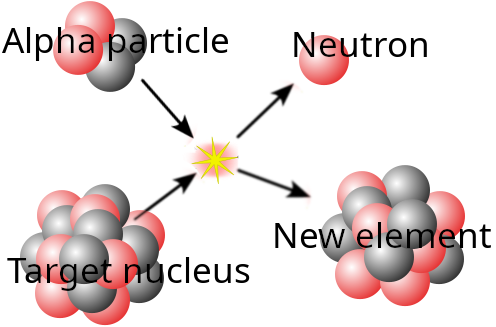
\includegraphics[width=0.55\textwidth]{anreaction.png}
	\caption{Illustration of an \an reaction.}
	\label{anreaction}
\end{figure}

\section{Relevance of \an reactions}
Underground experiments trying to detect dark matter WIMPs or other rare events have to deal with neutron backgrounds that are hard to distinguish from the desired particles.

This is because, in the case of WIMPs, they are hypothetical neutral particles, that interact with matter exclusively through nuclear reactions (and gravity).
A successful WIMP detection could easily be confused with neutrons.
In order to reduce this background, such experiments go deep underground, where cosmic rays and the particles they create are absorbed by the earth.
\\

However, neutrons are still produced underground, both by spontaneous fissions and by \an reactions (from $\alpha$ decay), and so they still have to deal with a background, albeit smaller.
This background dominates over the one produced by cosmic rays at depths higher than \qty{1}{\kilo\meter}.
The main contribution to \textbf{this} background comes from \an reactions, produced by $\alpha$ particles coming from the radioactive decay of elements in the ground and in the detectors themselves.\cite{neutron_in_an}

A good knowledge of the yield of these reactions and of the neutron spectra they produce is thus useful to differentiate between background counts and rare events.
Better data can improve monte carlo simulations, and lead to more sensitive detectors.
\\

\begin{figure}[H]
	\centering
	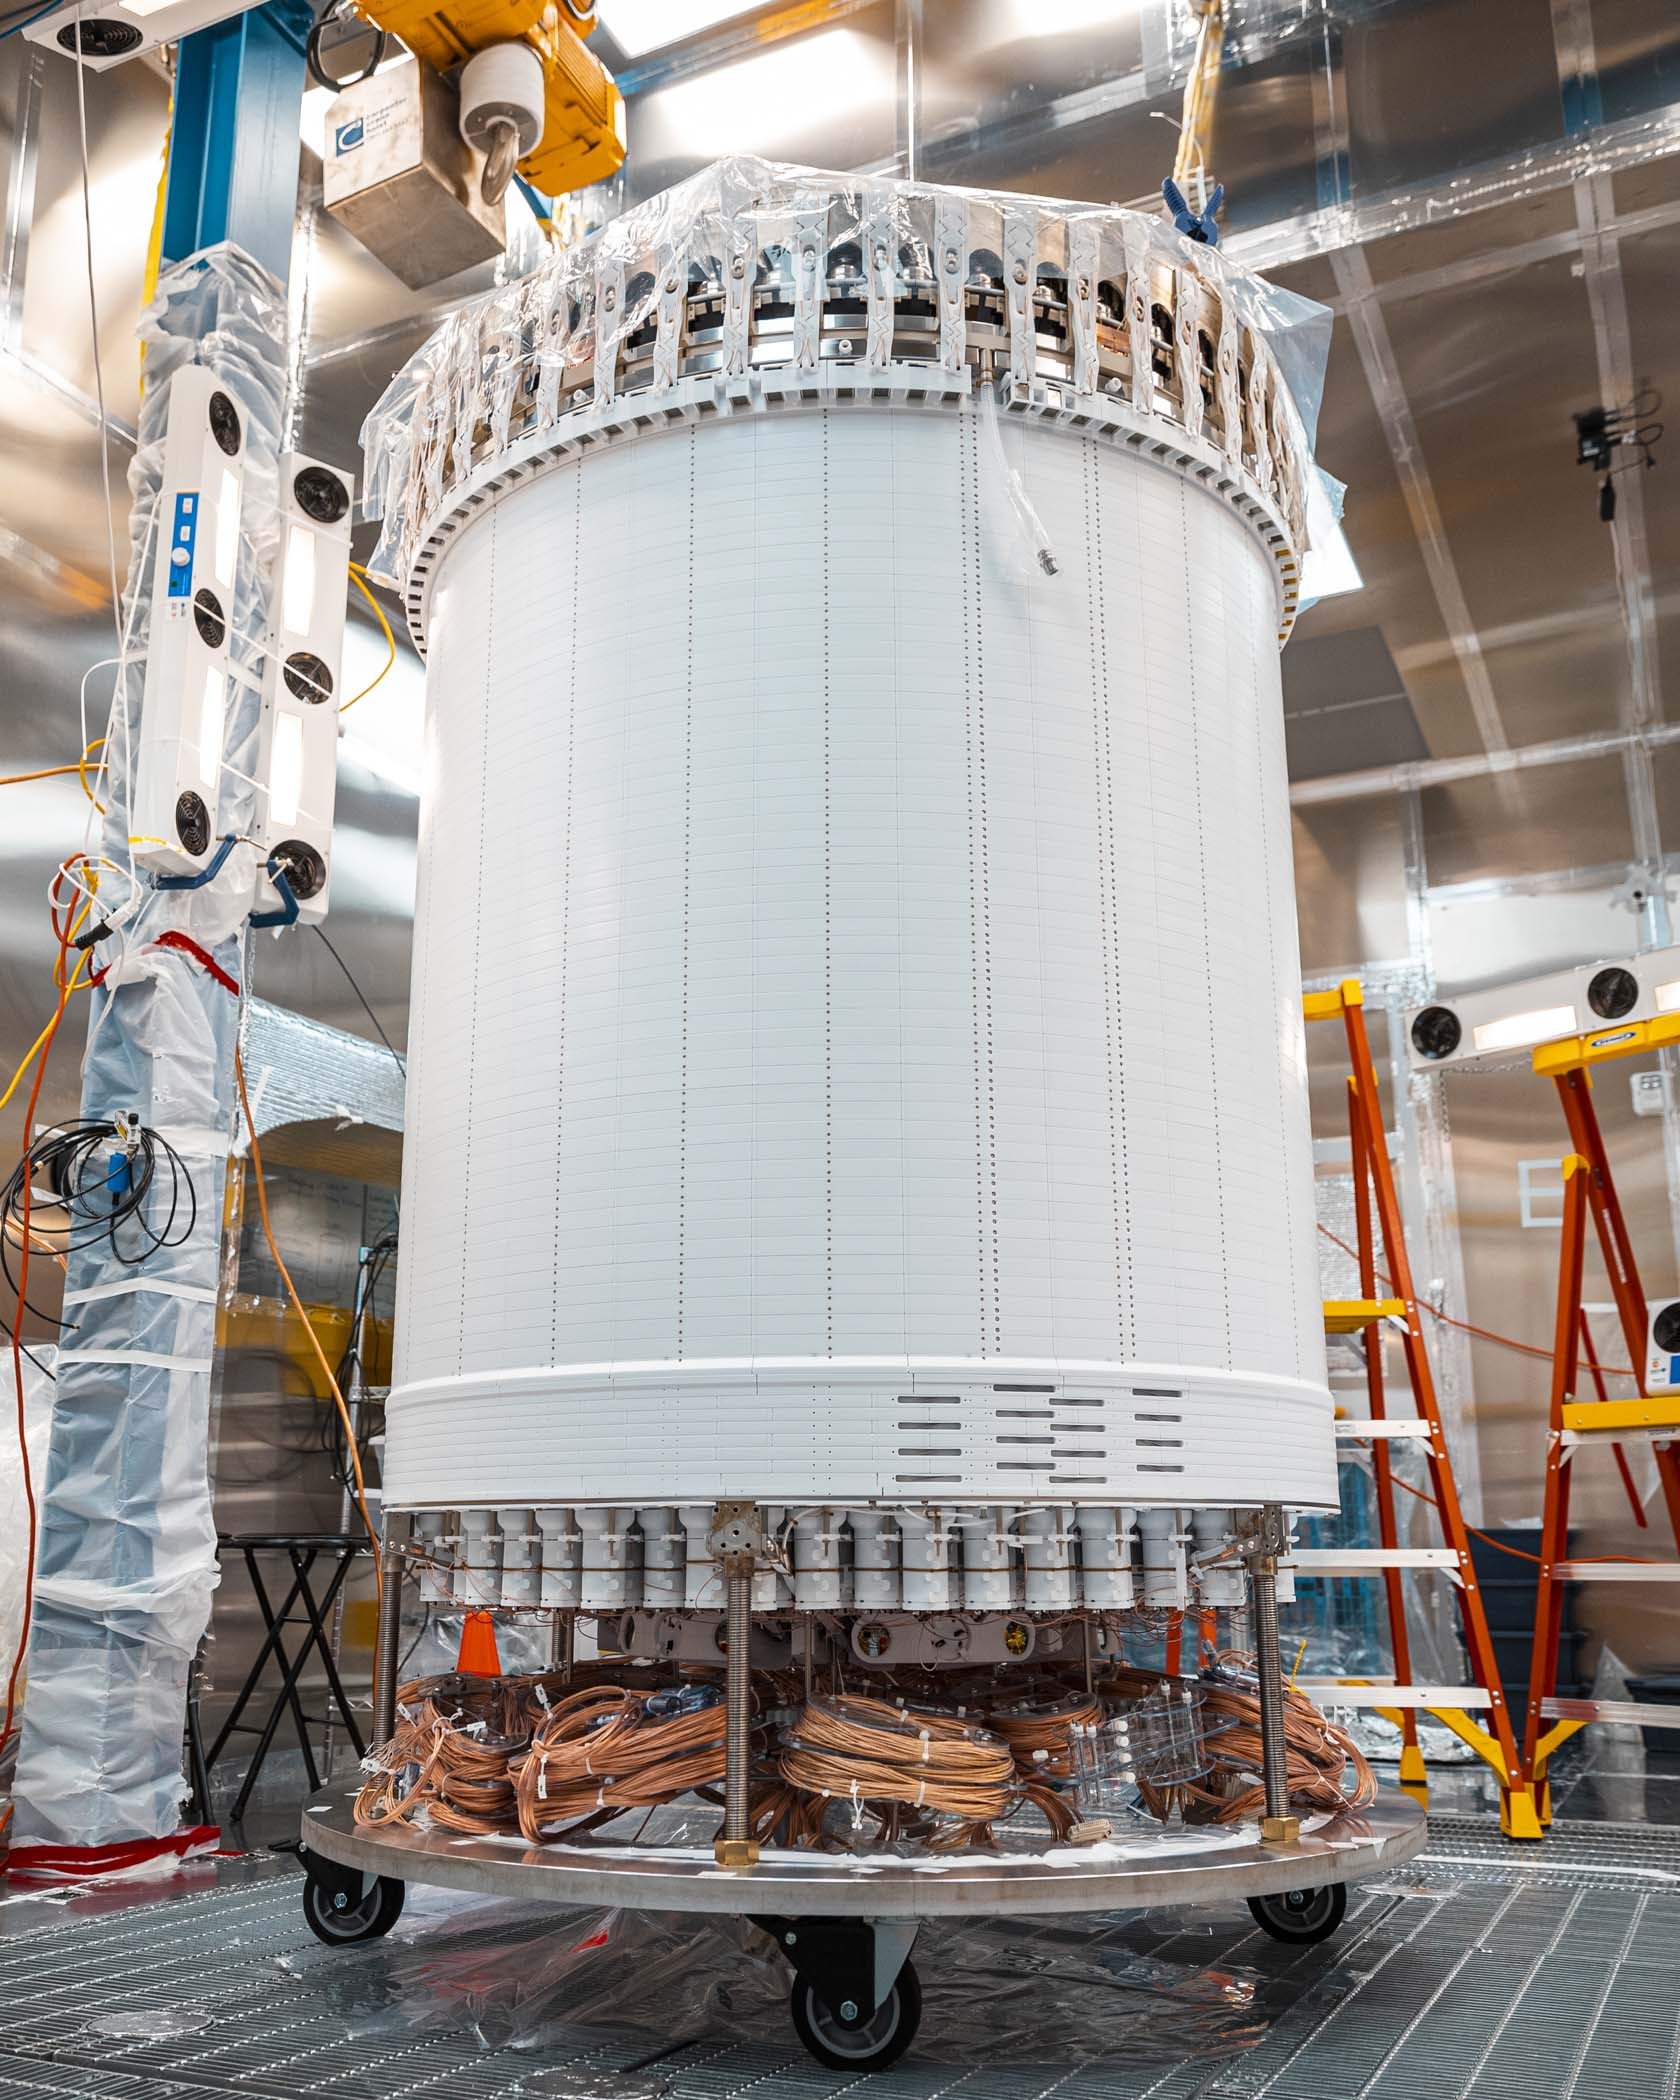
\includegraphics[width=0.5\textwidth]{sanford.jpg}
	\caption{The LUX-ZEPLIN experiment, situated \qty{1.5}{\kilo\meter} underground at the Sanfor Underground Research Facility in the U.S., is an experiment currently taking data in the search for WIMPs by using xenon detectors.
	Source: \href{https://sanfordlab.org/experiment/lux-zeplin}{sanfordlab.org}}
	\label{sanford}
\end{figure}

\an reactions are also of interest in astrophysics, as they are the main source of neutrons for the s-process and very important for the synthesis of elements.\cite{astro1}\cite{astro2}
Other fields of interest include fission and fusion reactors and assays for non-proliferation and spent fuel management.\cite{INDC}

\section{Actual state of \an measurements and objective at CNA/HiSPANoS}
Most of the \an reactions data was measured decades ago, is incomplete, and/or the uncentainties in cross sections and produced neutron spectra are very large.
Previous measurements were carried out mostly through \textit{activation} measurements or with moderated neutron counters, meaning there is little data on the energy spectra of produced neutrons.
Improved data is needed, and many groups are in the process of doing measurements.\cite{INDC}
\\

The purpose of this work is to study the viability of doing measurements of \an reactions using the neutron line at the CNA's \qty{3}{\mega\volt} acelerator, as part of the MANY collaboration \cite{MANY}\cite{hispanos}.
It can achieve $\alpha$ particles of up to \qty{9}{\mega\eV} (more details in the next chapter), which covers the range of interest for underground experiments.\cite{CNA}

In order to carry out this test, this work will study \an reactions in \Aliso: which is the standard material for such measurements and has the best yield data to compare to.
If successfull, measurements of \an reactions in other materials can be carried out in the future.
\\

\begin{figure}[H]
	\centering
	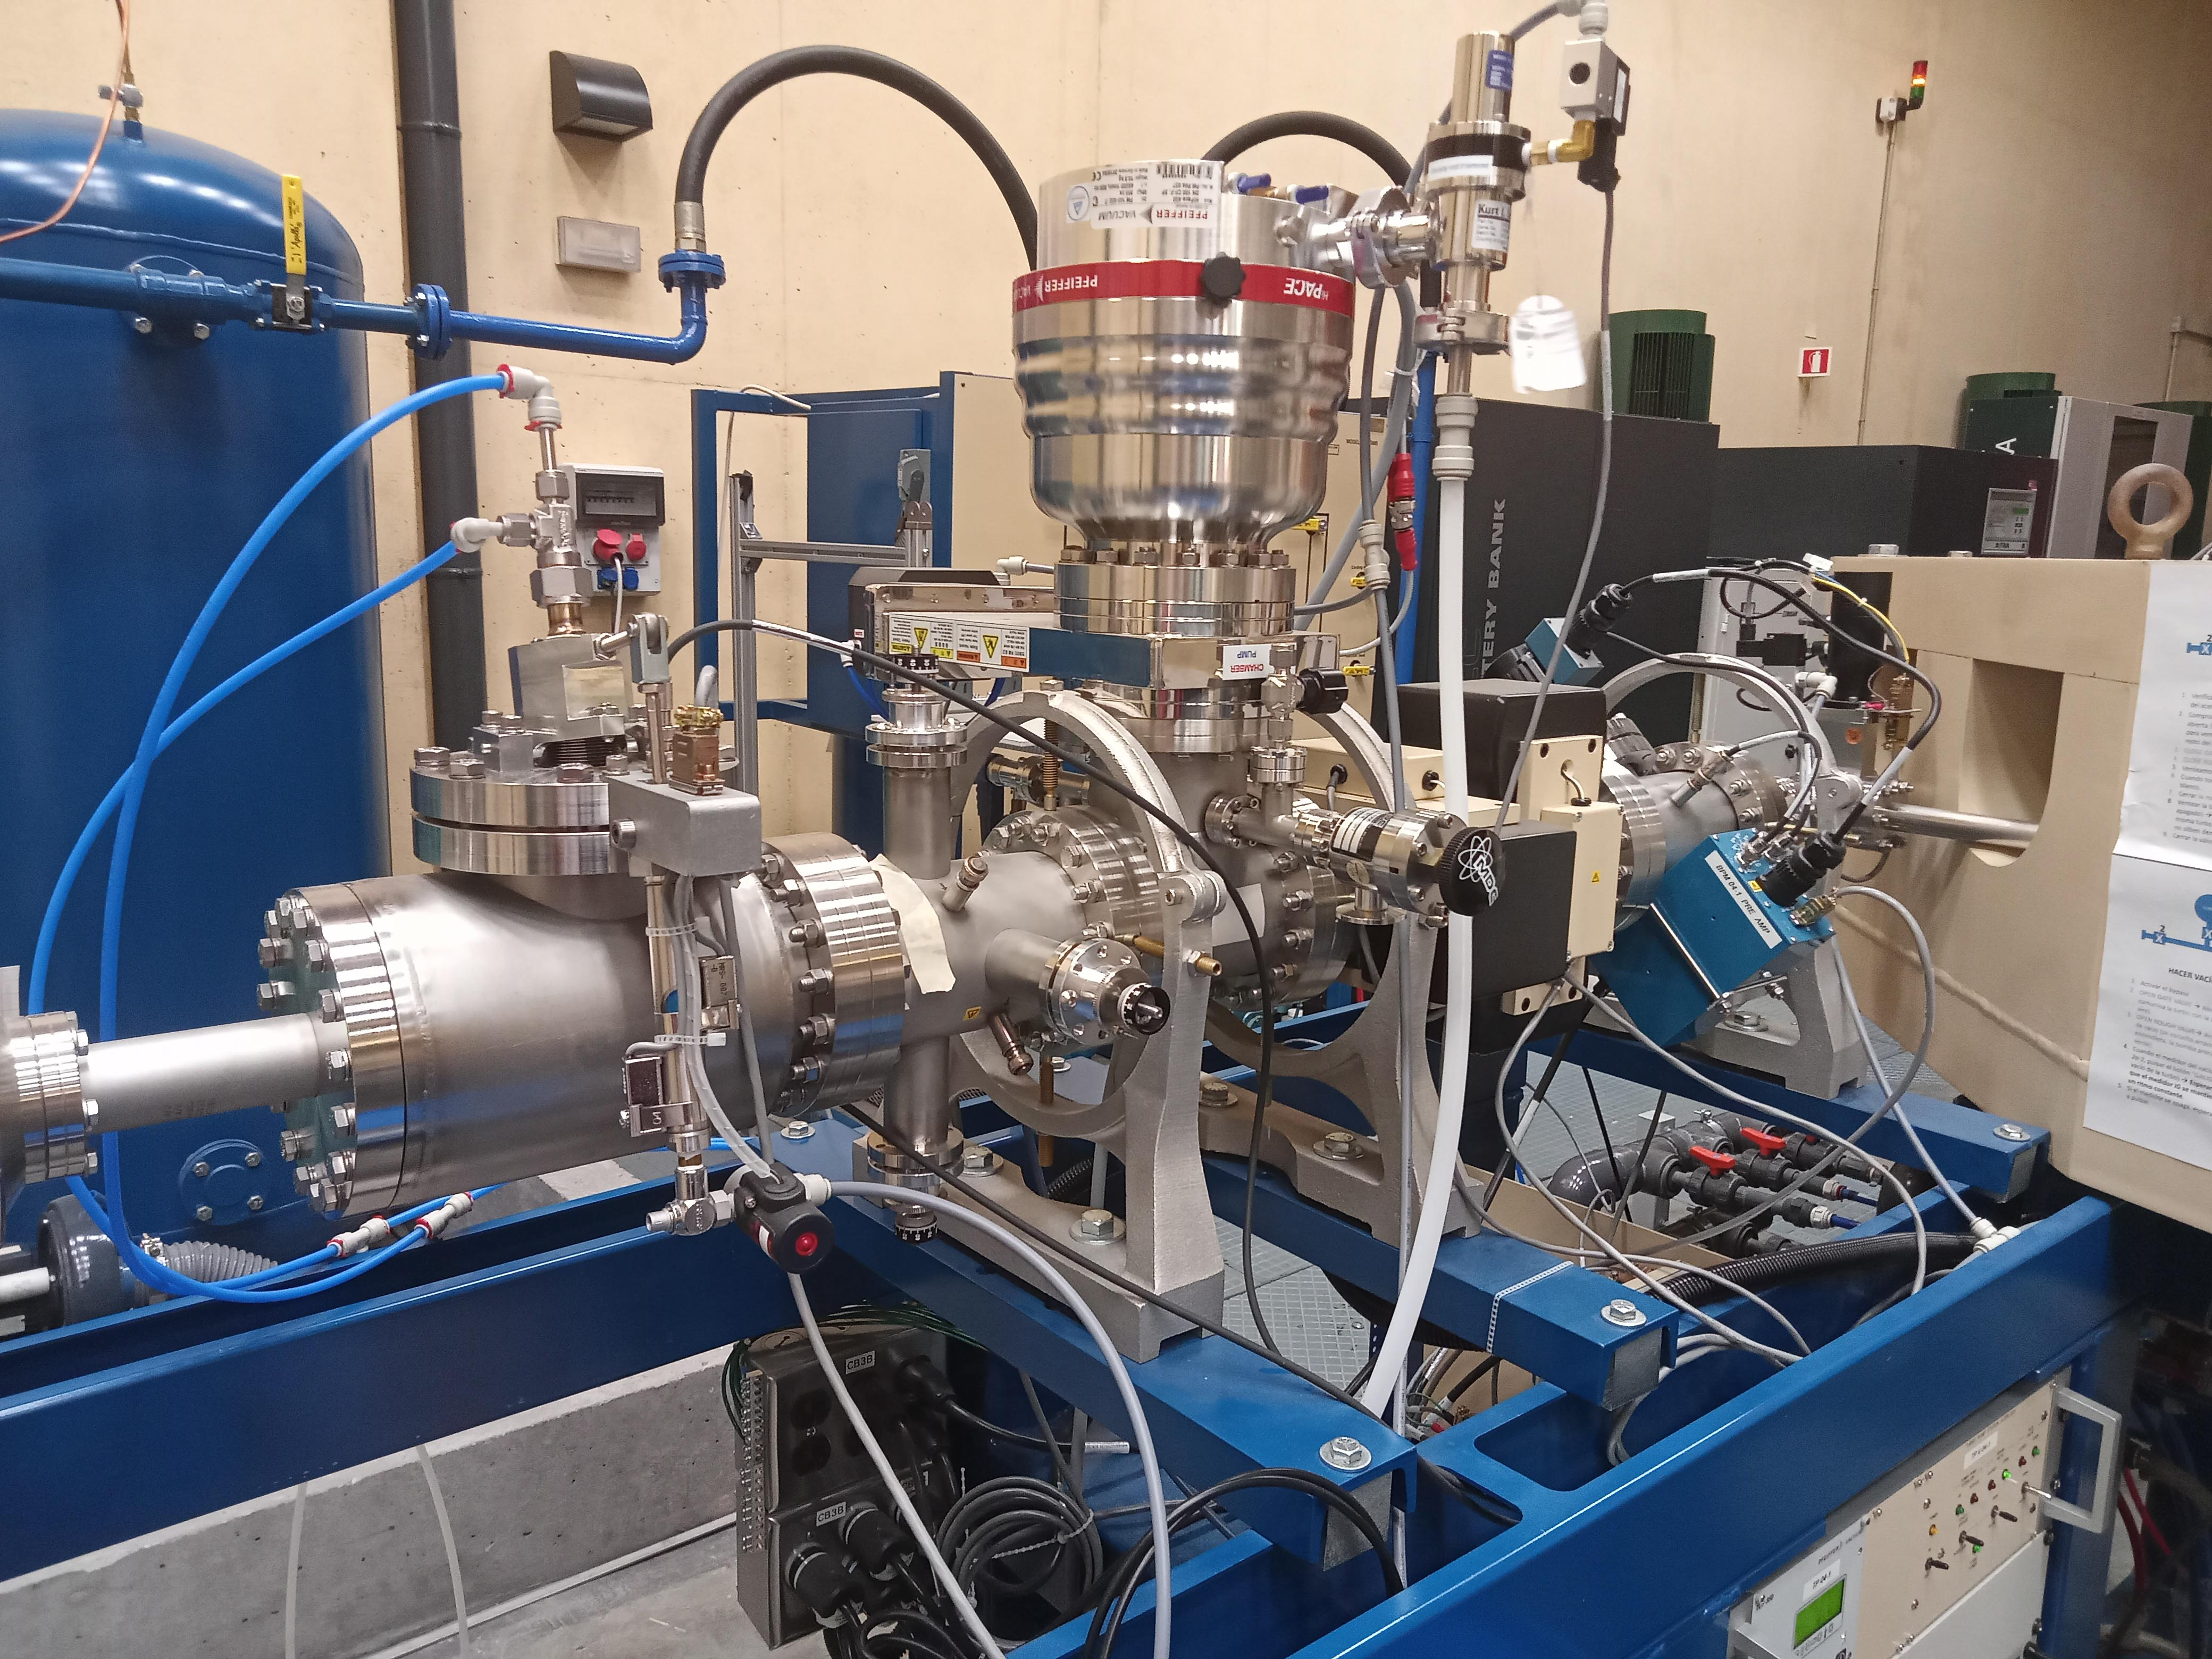
\includegraphics[width=0.6\textwidth]{neutronline_foto.jpg}
	\caption{Picture of the CNA/HiSPANoS neutron line, used in this work.}
	\label{neutronline_foto}
\end{figure}

We will measure both the \textit{thick target yield} of the reaction, as well as the energy spectra of the produced neutrons.
For the yield, we will do \textit{activation} measurements, where we measure the decay of the radioactive product produced by the reaction.
Lastly, for the energy spectra, we will do \textit{pulsed beam} measurements, and determine the produced neutron's energies via \textit{time-of-flight}.
\\

The literature data we will compare our results to come from \textit{G. J. H. Jacobs and H. Liskien}, from 1983.\cite{jacobs}
It presents thick target yield data for a larger energy range than this work will study, and agrees well with other measurements in the literature.\cite{jacobssupport1}\cite{jacobssupport2}
The data is shown in a table, but also uploaded to the EXFOR database.

It also gives the energy spectra of the produced neutrons at \qty{5.5}{\MeV} at \qty{60}{\degree}, the only available prior measurement of \Aliso\an neutron spectra we can compare to.
The data is presented in the form of a plot, from which numbers were obtained.


\chapter{Experimental setup}
The measurement of \an reactions required a beam of $\alpha$ particles, a suitable target, and radiation detectors to observe either the neutron emitted in the reactions or the $\gamma$-rays emitted by the decay of the reaction product.
The beam of $\alpha$ particles is delivered by the \qty{3}{\mega\volt} tandem accelerator at CNA.
The target is a high purity thick \Aliso disk.
The detectors used are both organic (for neutrons) and inorganic (for $\gamma$-rays) scintillators placed around the target, at different distances and angles.

They are all connected to a data acquisition system (DAQ), that records every signal for offline analysis.
The current hitting the target is also monitored, by a charge integrator also connected to the DAQ.

\begin{figure}[H]
	\centering
	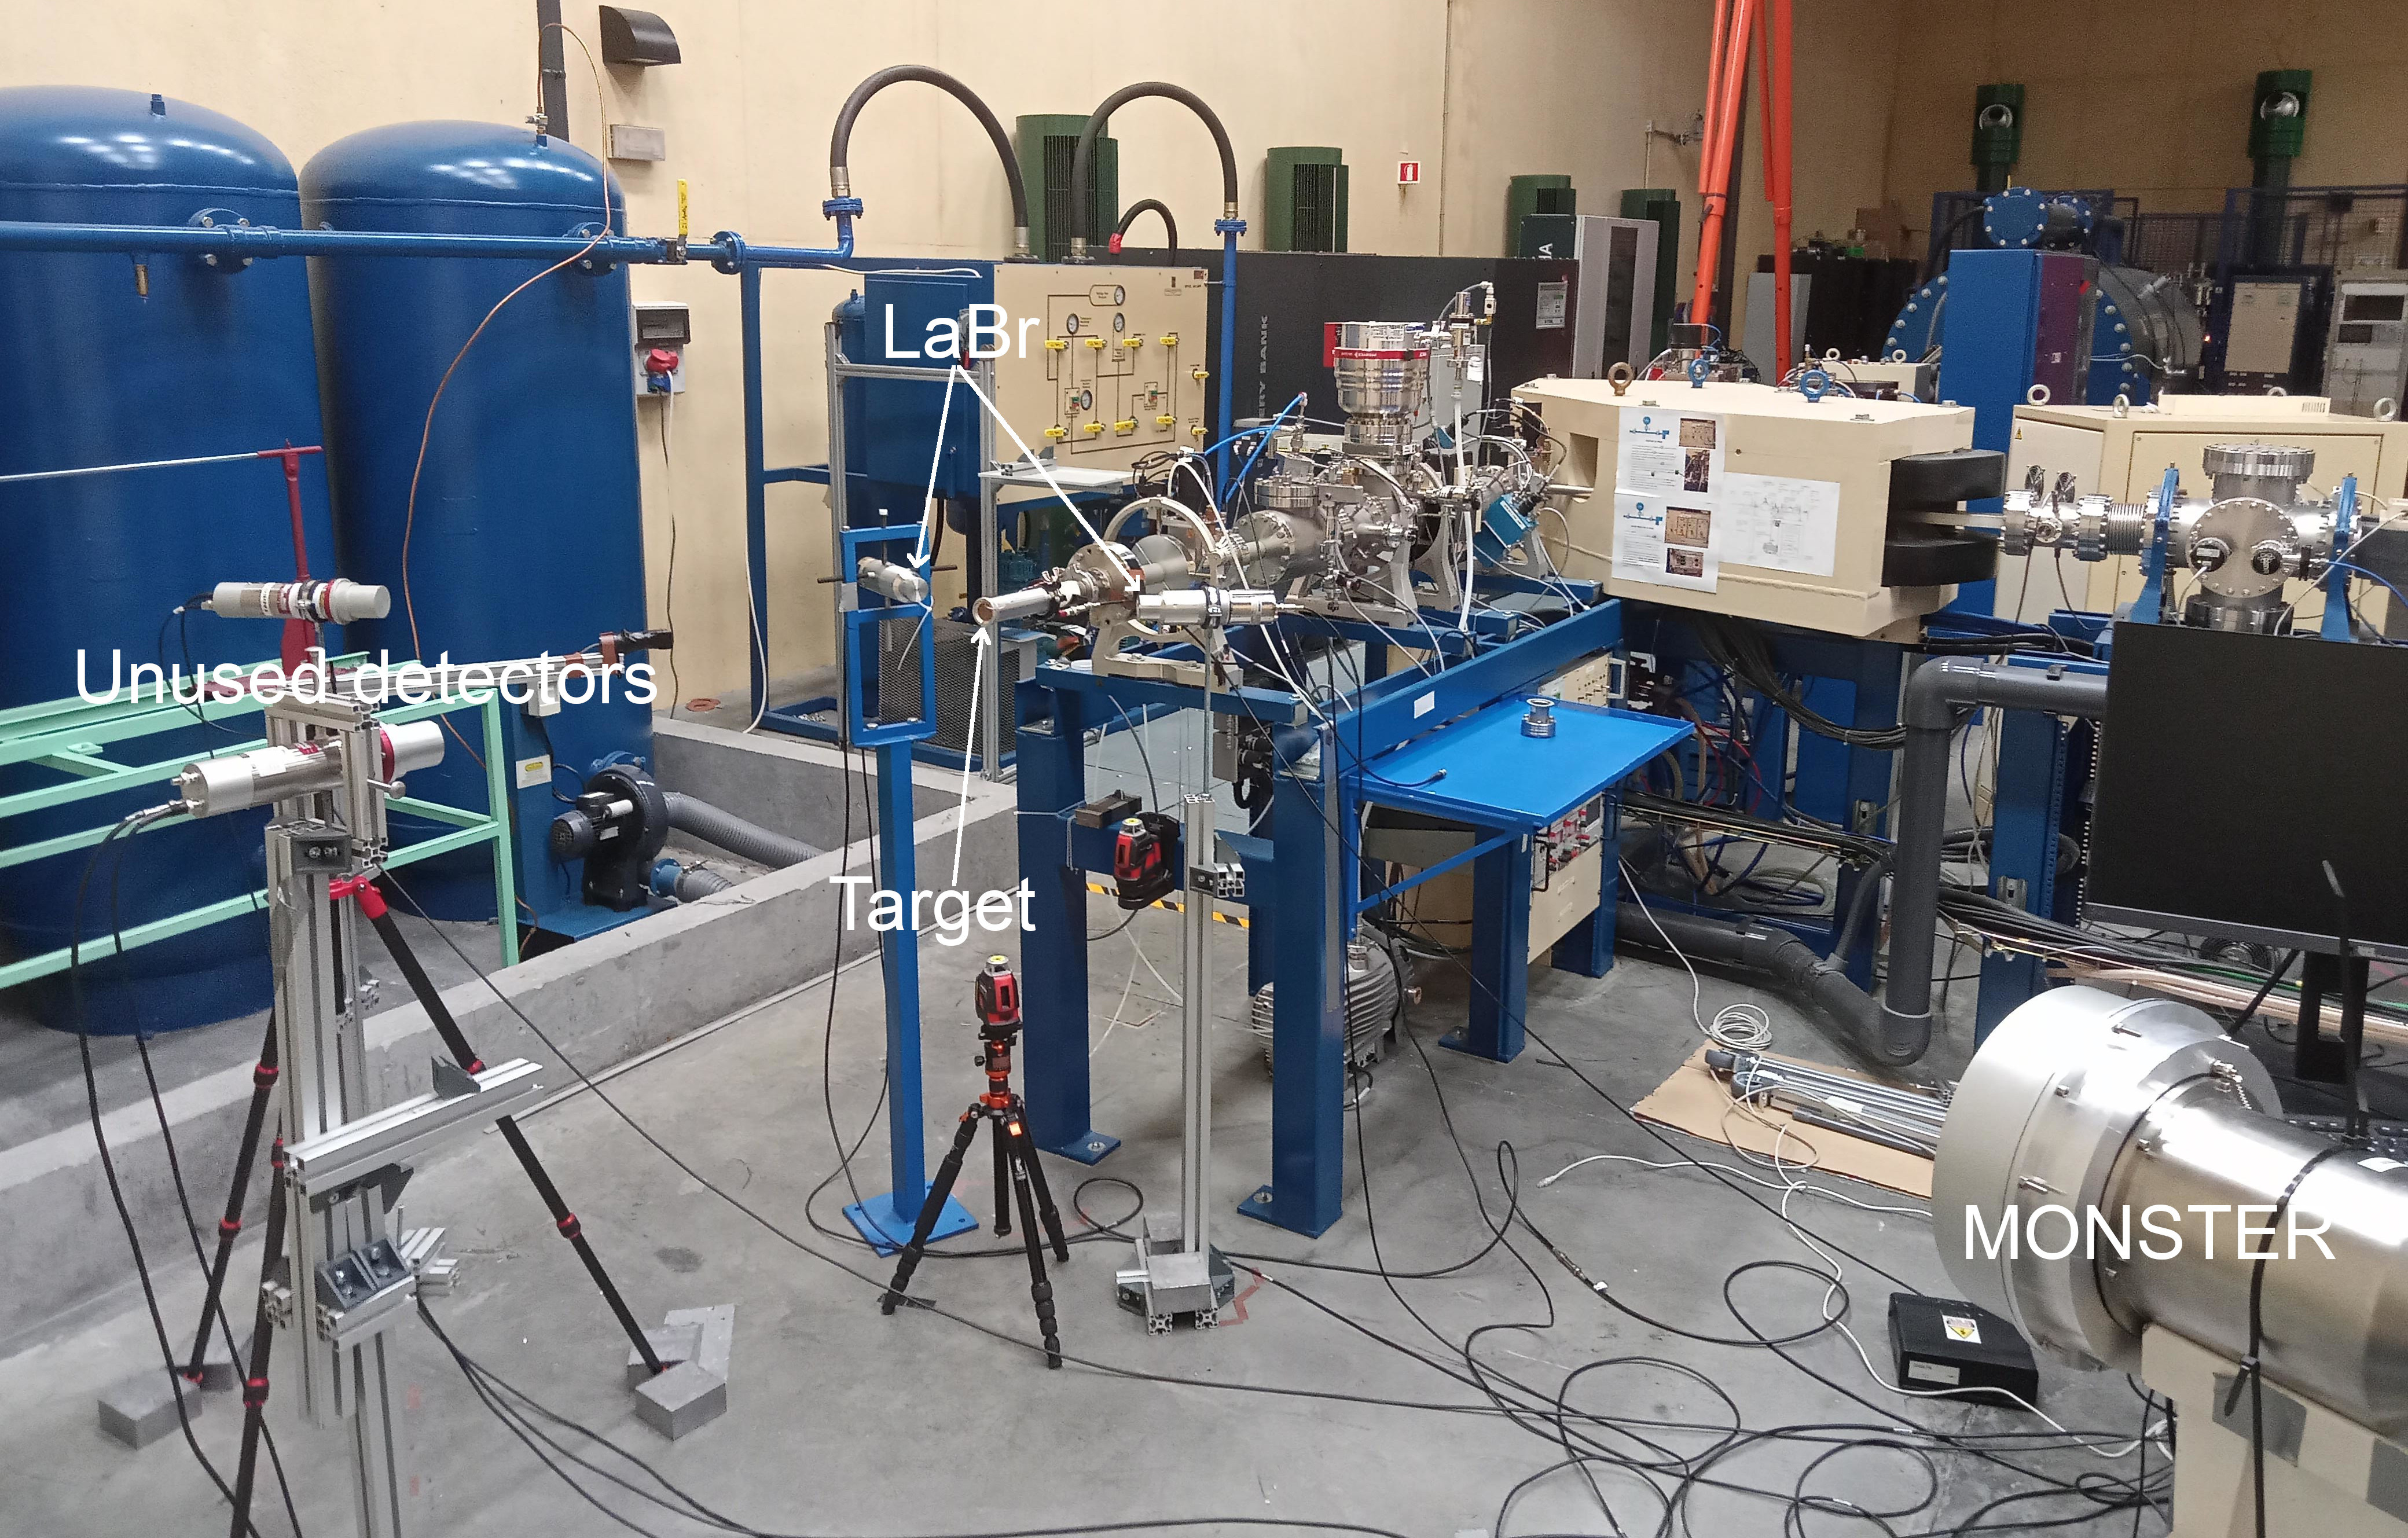
\includegraphics[width=0.80\textwidth]{overview_photo.jpg}
	\caption{Overview picture of the experimental setup.
	Detectors and the target are labeled.}
	\label{overview_photo}
\end{figure}

\section{Tandem 3MV accelerator}
A tandem is a type of linear particle accelerator whose main characteristic is that particles are accelerated twice by the same terminal voltage.
Particles are injected with negative charge from a source situated outside the tank, and accelerated toward the terminal.
Once the negatively charged particles arrive at the terminal, their electrons are removed by a gas, called the \textit{stripper}.

Now with a positive charge, they are accelerated the rest of the way by the same voltage.
\\

In the case of $\alpha$ particles, they are injected with charge state -1 and then stripped of all electrons, to charge +2.
Given that the maximum voltage of the CNA tandem accelerator is \qty{3}{\mega\volt}, they can be accelerated to a maximum of $3\cdot\left(1+2\right) = \qty{9}{\mega\eV}$ plus the injection energy, which is about \qty{70}{\keV} depending on the source.
\\

\subsection{Pulsed beam mode}
For most applications, the accelerator generates a continuous stream of particles.
But it can also be operated in a \textit{pulsed beam} manner, where particles are emitted in groups, or \textit{pulses}.

Ideally, those pulses are instantaneous: all particles arrive to the end of the beam, where the target is placed, at exactly the same time.
In reality, they are approximately a gaussian distribution, with a certain width in the order of about \qty{2}{\nano\second} nanoseconds.
\\

To achieve pulsed operation, the accelerator uses two devices: the \textit{chopper} and the \textit{buncher}.
The \textit{chopper} generates an electric field that deflects all particles coming from the accelerator.
With a frequency of choice between \qty{32}{\kilo\Hz} and \qty{2}{\mega\Hz}, it disengages the field and lets particles pass for a time period of choice, between 40 and \qty{250}{\nano\second}.

After the chopper, the \textit{buncher} uses further electric fields to slow down the faster particles and accelerate the slower ones, making the pulse narrower in time (\qty{2}{\nano\second}) and Gaussian shaped.\cite{hispanos}
\\

\subsection{Difficulties with accelerating $\alpha$ particles}
Although it is used in this experiment to pulse $\alpha$ particles, the CNA Tandem buncher was not designed for them.
Rather, it was designed to pulse beams of only protons and deuterons, the latter having the same mass-to-charge ratio as $\alpha$ particles.
However, the electric fields used by the buncher to shape pulses are not strong enough for $\alpha$ particle beams with the energies that the beam injector can provide.

The consequence is that the pulses of $\alpha$ particles feature a Gaussian peak with only a few \unit{\nano\second}, but with a sizable fraction of the beam arriving at later times, creating a tail (see Figure \ref{uneven_gflash}).
This affects the neutron energy resolution that can be achiveed in time-of-flight measurements, being part of the objective of this work to study this limitation.
\\

\subsection{The HiSPANoS neutron beam line}
After the particles are accelerated, they pass through the neutron line before hitting the target.
This is placed after the accelerator's \qty{90}{\degree} analyzing magnet, typically used to deflect particles toward the other experimental lines.

Because the neutron line is parallel to the accelerator, the magnet cannot be used to select particles (discard particles that do not have the desired charge state/speed ratio), for instance $\alpha$ particles that have lost only 1 electron in the stripper.
This is done instead by the Wien filter placed in the beam line.
However, the amount of $\alpha$ particles with charge +1 is negligible at the terminal voltages used in this work.
\\

Figure \ref{tandemdiagrama} shows an schematic view of all the beam components and the experimental set-up used in this work.

\begin{figure}[H]
	\centering
	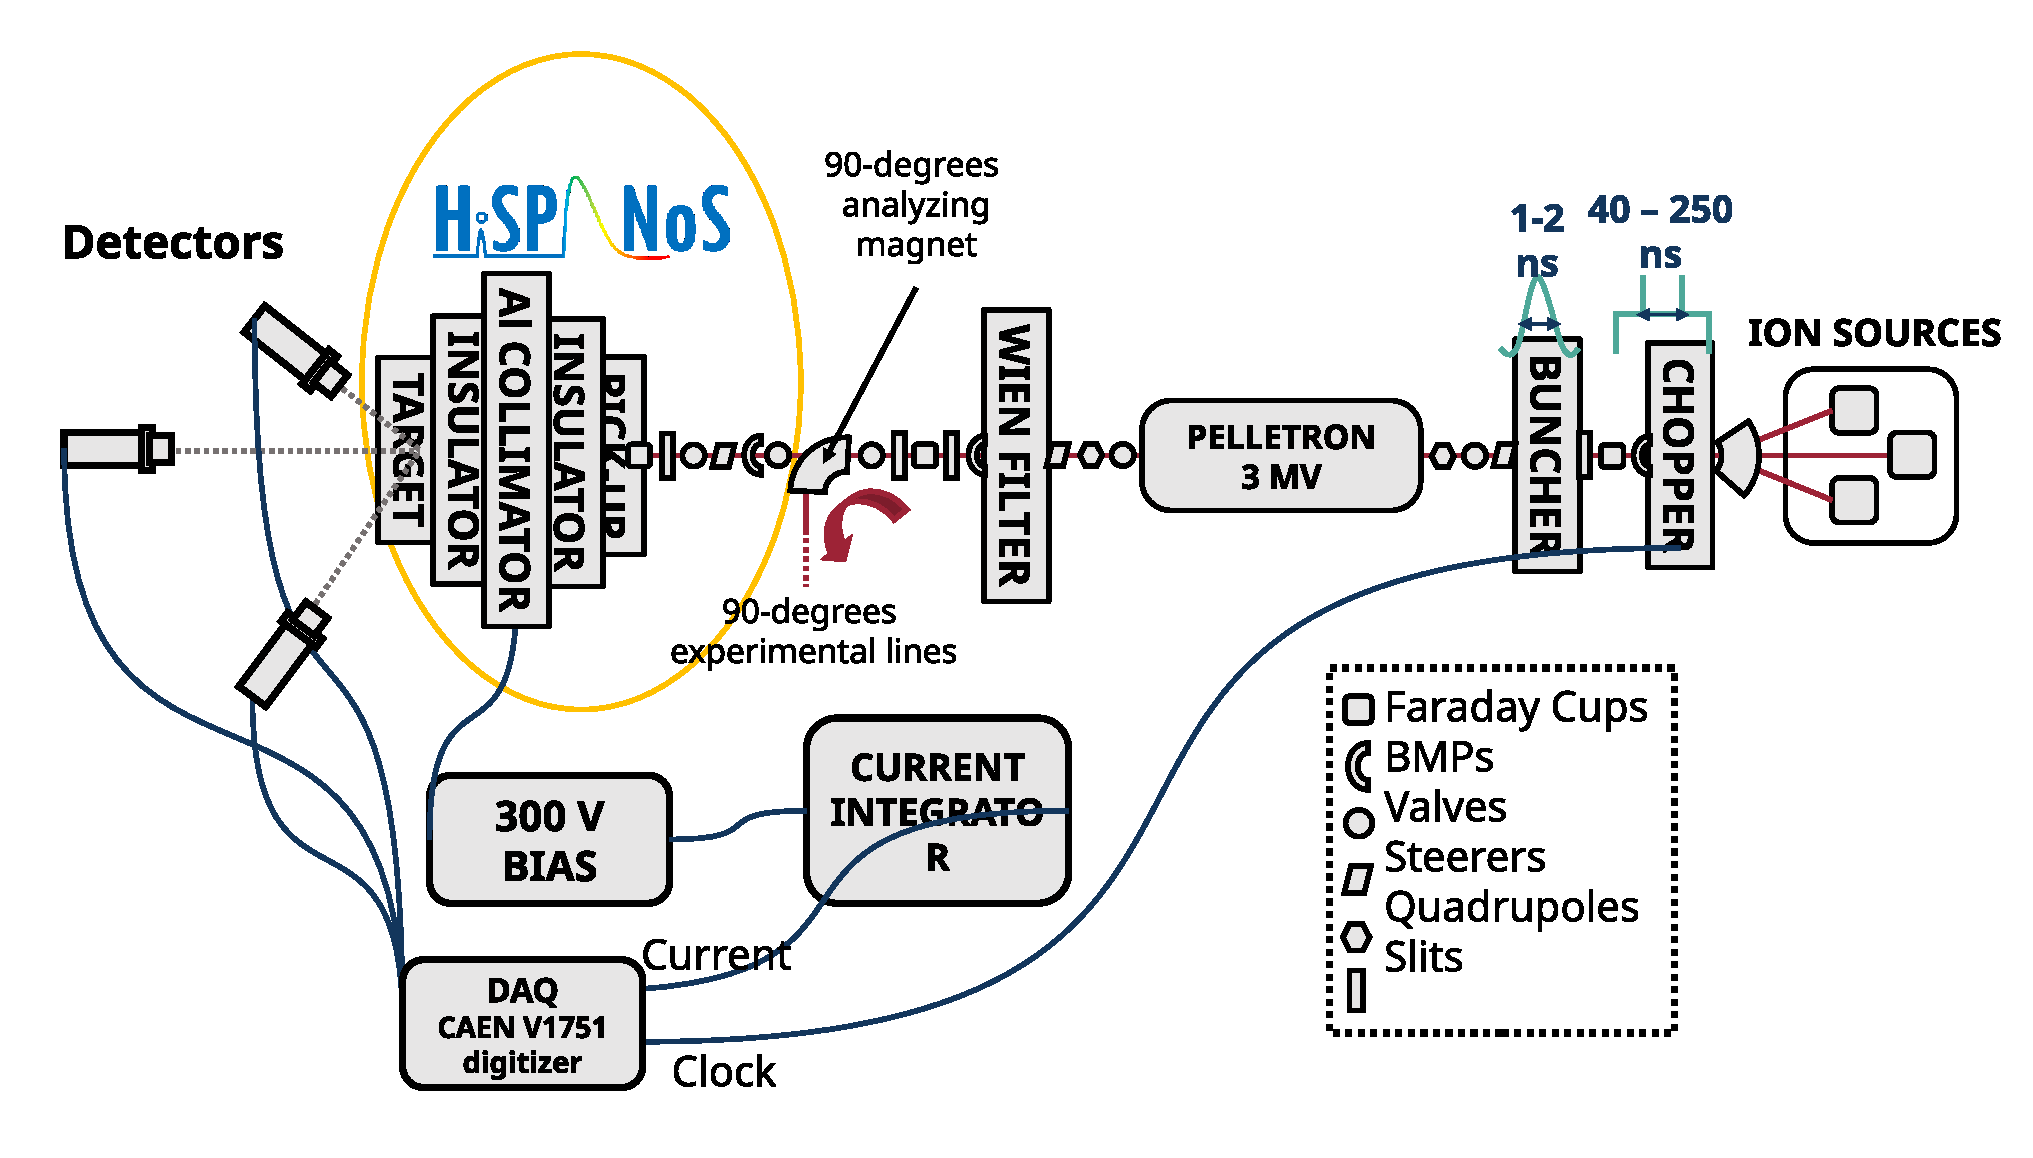
\includegraphics[width=0.90\textwidth]{tandemdiagrama.eps}
	\caption{Diagram of the accelerator system and HiSPANoS neutron line, with all components.}
	\label{tandemdiagrama}
\end{figure}

\section{The \Aliso target}
The target is a sheet of \qty{95}{\percent} purity \Aliso.
Since the range for 9~MeV $\alpha$ particles is around \qty{380}{\micro\m} in aluminum, the few \unit{\mili\m} thich target is enough to be considered a thick target, meaning it will stop all incoming $\alpha$ particles.
\\

\section{Beam current monitoring}
It is important, in order to obtain quantitative results, to know how many $\alpha$ particles hit the target.

The target is electrically isolated from the rest of the neutron line by insulators (Figure \ref{tandemdiagrama}), and so it charges up positively as $\alpha$ particles impact it.
By measuring the charge on the target, we can know how many $\alpha$ particles were incident.
To do so, we connect the target via a cable to a ORTEC 439 Digital Current Integrator module, a \textit{charge integrator} that emits a pulse and discharges the target each time it reaches \qty{0.1}{\nano\coulomb}, or approximately \num{3E8} $\alpha$ particles.
In order to suppress the secondary electrons emitted from the target when the beam hits it, the last fraction of the beam hosts a large diameter collimator that is set to \qty{-300}{\V} and hence pushes these electrons back to the target.

\begin{figure}[H]
	\centering
	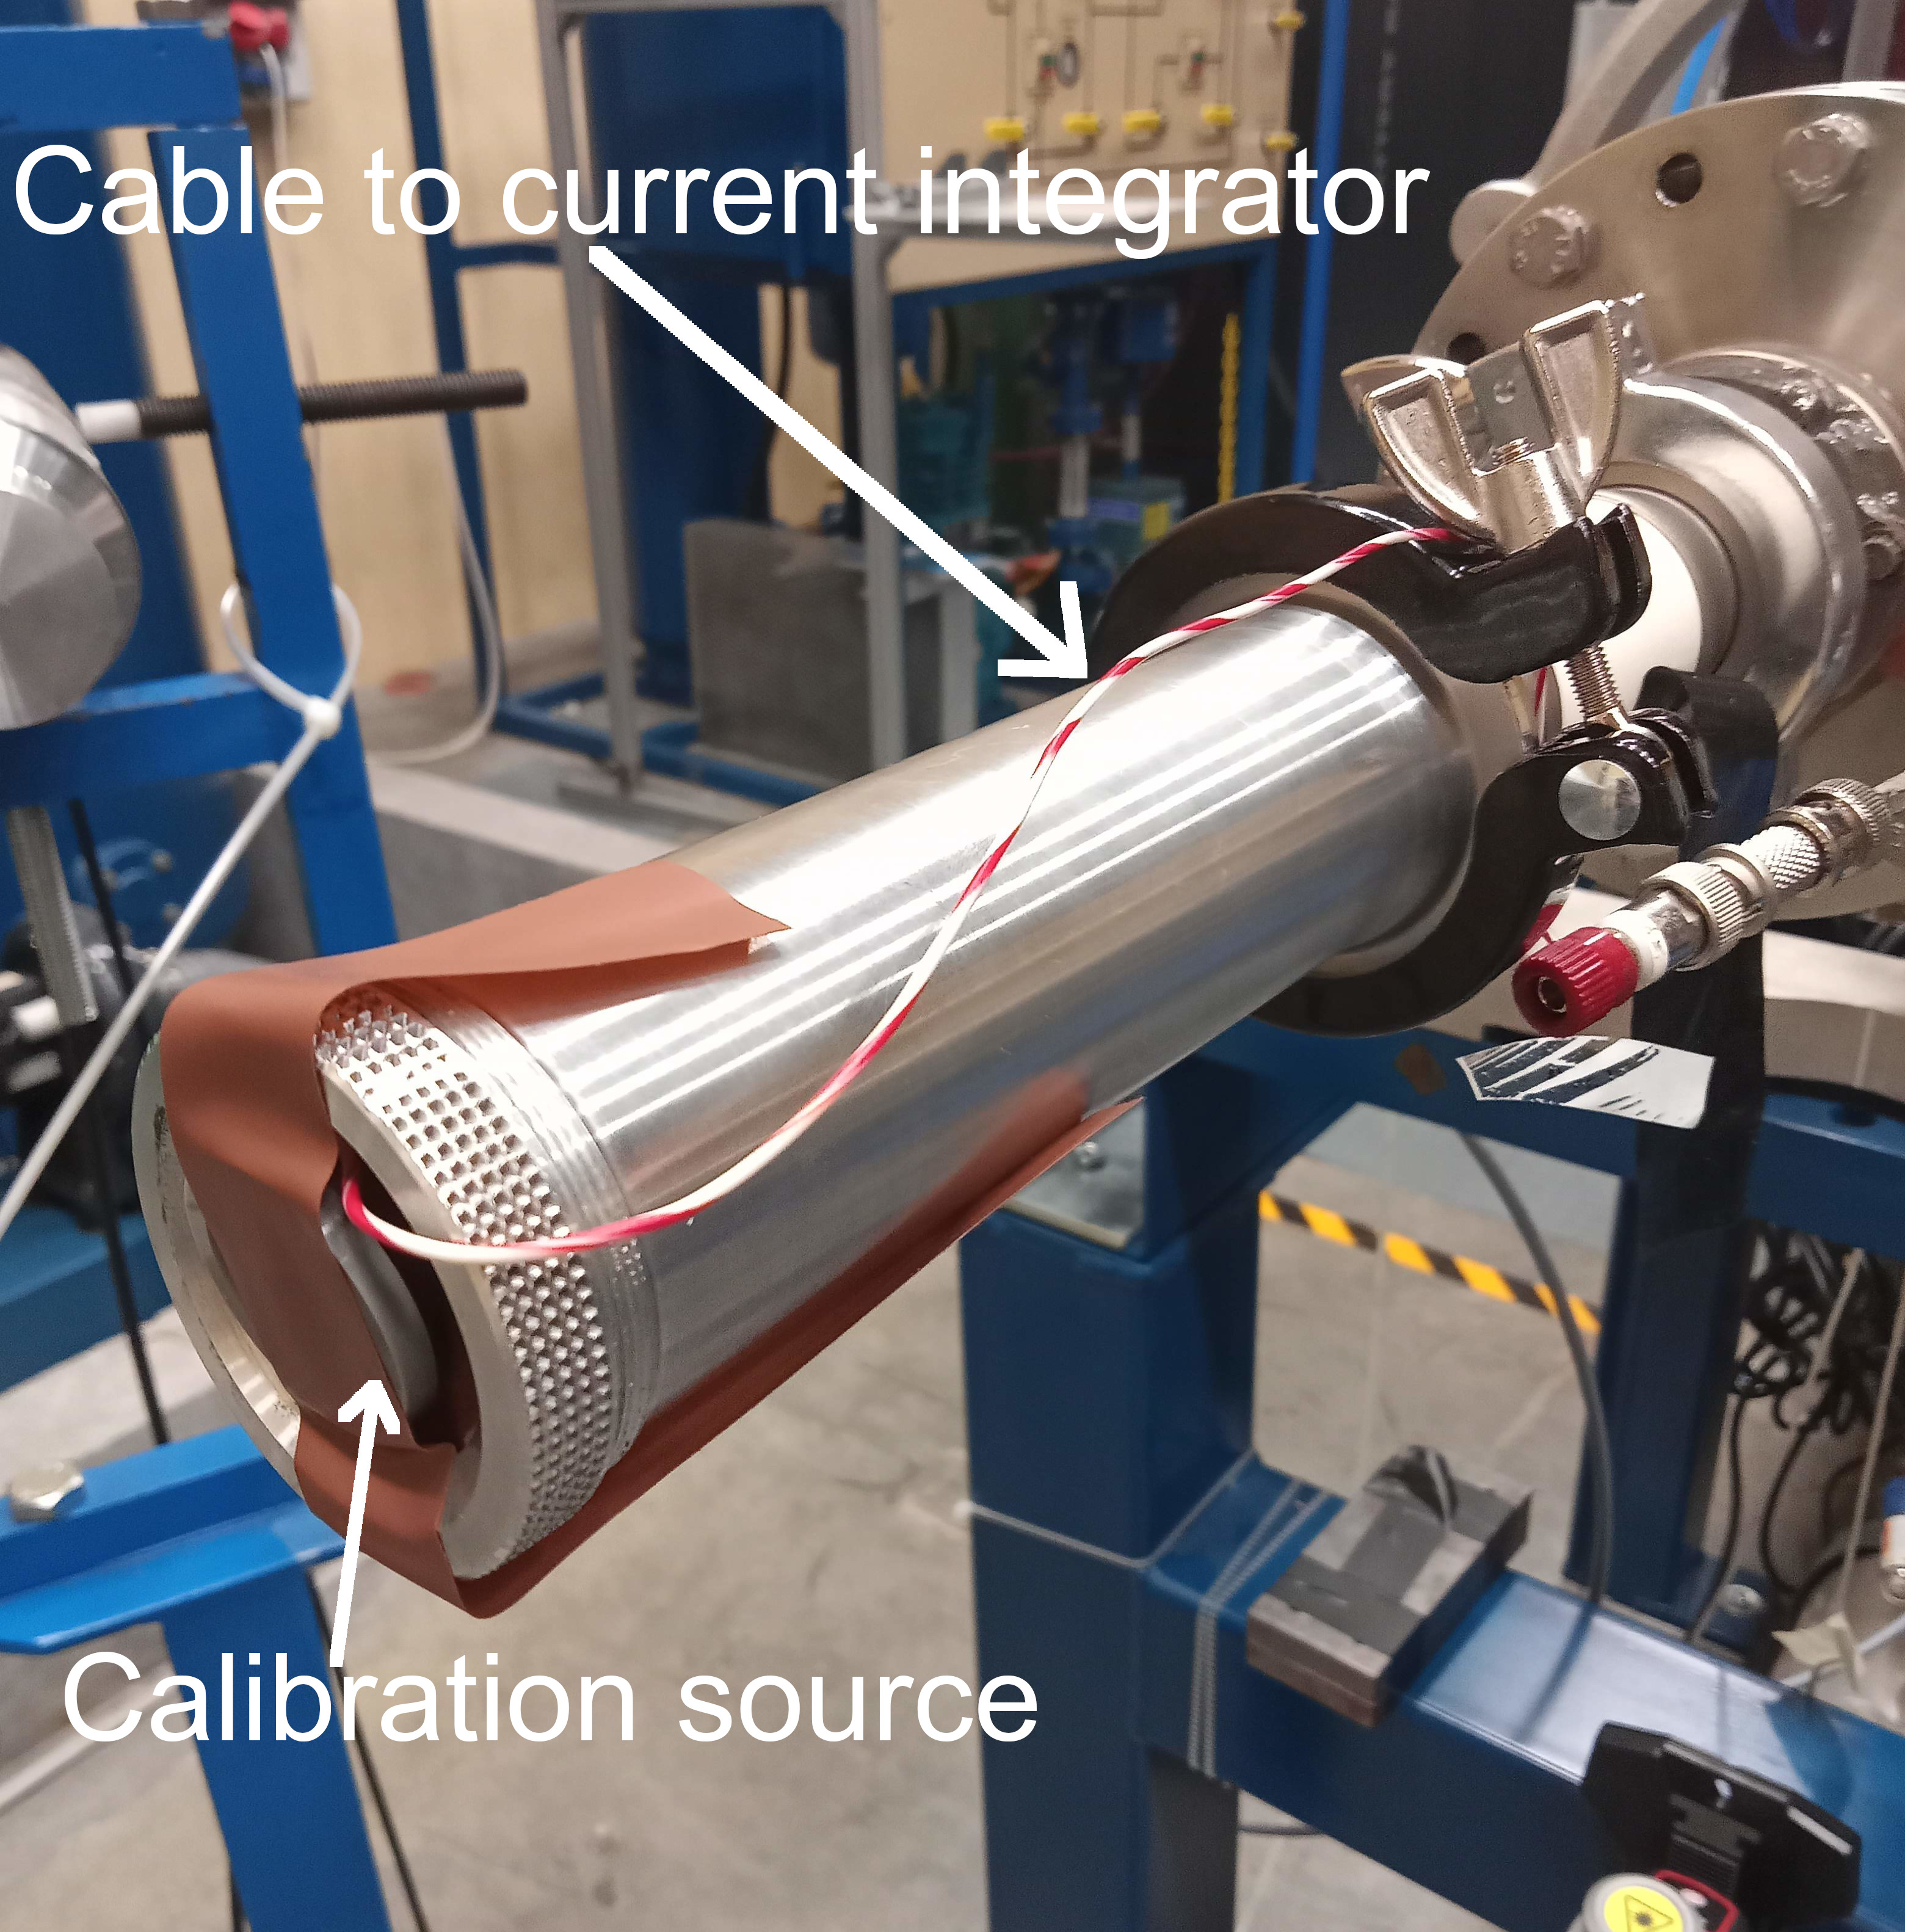
\includegraphics[width=0.5\textwidth]{target_with_calibration.jpg}
	\caption{Target at the end of the neutron line, with a calibration source taped for efficiency calibration measurements.}
	\label{target_photo}
\end{figure}

\section{Neutron and $\gamma$-ray detectors}
The Thick Target Yield (number of \an reactions per number of incident $\alpha$ particles) is measured by activation using $\gamma$-ray detectors, while the \an neutron spectra is measured via time-of-flight measurements using a neutron detector.
\\

\begin{table}[H]	%Tabla con distancias y ángulos de detectores
\centering
\begin{tabular}[c]{>{\bfseries}l||c|c}
	Detector		& Distances\tablefootnote{Detectors were moved in order to get measurements at different distances. For the LaBr\textsubscript{3} detectors, their distance was not measured with precision.} (\unit{\cm})& Angle\\ \hline
	\textbf{MONSTER}	&\num{100}, \num{200}		&\qty{60}{\degree}	\\ \hline
	\textbf{LaBr\textsubscript{3}(1)}		&\num{20} to \num{30}		&\qty{150}{\degree}	\\ \hline
	\textbf{LaBr\textsubscript{3}(2)}		&\num{20} to \num{30}		&\qty{-150}{\degree}	\\ \hline
\end{tabular}
\caption{Angles and distances of detectors.}
\label{distances_angles_table}
\end{table}

\subsection{LaBr\textsubscript{3} detectors}
To measure $\gamma$-rays, we use two LaBr\textsubscript{3} (lanthanum bromide) detectors, which we refer to as LaBr\textsubscript{3}(1) and LaBr\textsubscript{3}(2).
They are inorganic scitillators, meaning they produce light when hit by ionizing radiation.
This can be used to detect gamma rays by the following process:

When a $\gamma$-ray hits the scintillator, it gives all of its energy via the photoelectric effect, or part of it through Compton scattering, to an electron in the medium.
This electron travels the scintillator, losing energy by promoting electrons from the valence to the conduction band.
When these decay back to the valence bad, they go trough the intermediate states created by the Ce with which it is doped, emitting scintillating light, to which the material is transparent.

This \textit{scintillating} light is directed to a photocathode, where it emits electrons via the photoelectric effect.
These \textit{photo-electrons} are multiplied in a \textit{photomultiplier tube} (PMT), and finally turned into an electric pulse, which is registered as a detection.

Because proportionality is maintained in each of those conversions, the result is a spectroscopic response, where more energetic gammas generate proportionately bigger pulses.\cite{labr}
\\

To calculate the detectors' efficiency to the \qty{511}{\keV} $\gamma$-rays following the $\beta^+$ decay from \Piso, we use a \Na source that we tape to the target, at the end of the neutron line and in contact with the aluminum target.
This is shown in Figure \ref{target_photo}.
By fitting the resulting peak in the energy deposited spectrum to a Gaussian plus a background, we obtain the number of detected photons per second.
We then divide by the total number of emmited photons (given the source's activity) to get the efficiency.
\begin{equation}
	\text{detector efficiency} = \frac{\text{counts per second}-\text{background}}{\text{total source emissions}}
\end{equation}
This is done for each measurement and detector during the activation measurements.
Also pictured are the responses to \textsuperscript{137}Cs and \textsuperscript{60}Co sources, although they weren't used for efficiency calculations, as we are only interested in \qty{511}{\keV} $\gamma$-rays.

\begin{figure}[H]
	\centering
	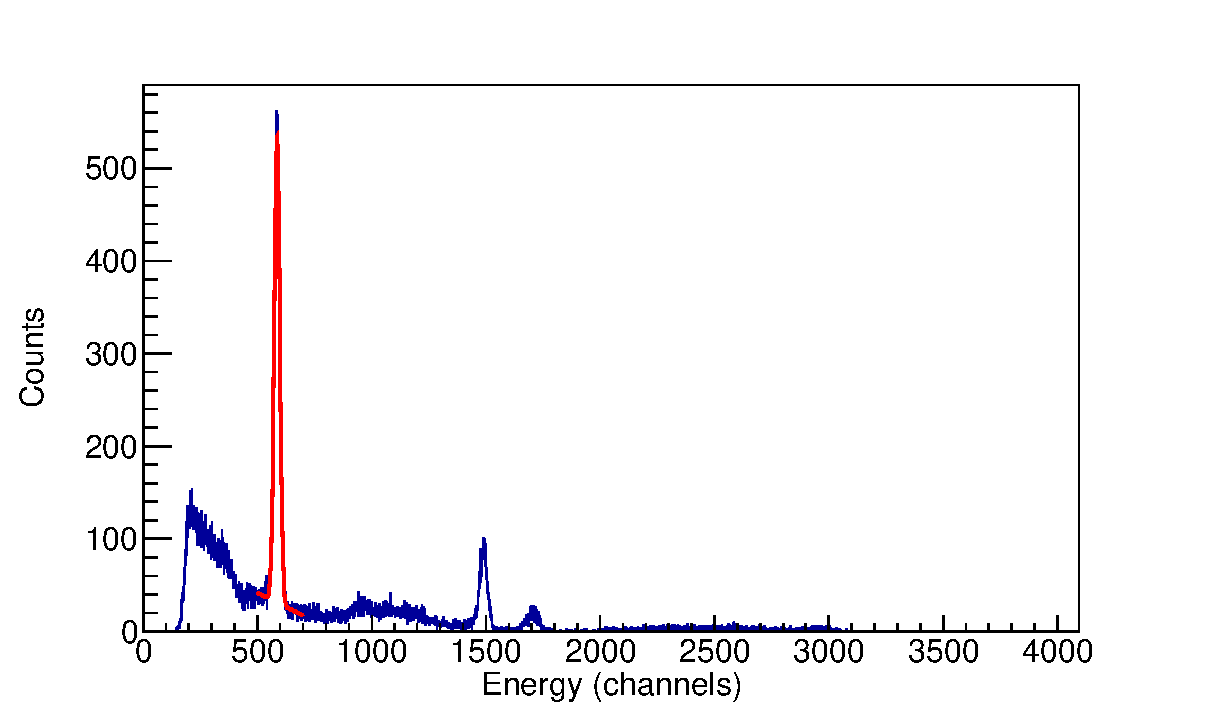
\includegraphics[width=0.80\textwidth]{labr_na22_calibration.eps}
	\caption{LaBr\textsubscript{3}(1) response to \Na source. In red is the fitting of the \qty{511}{\keV} peak to a Gaussian plus a linear background.}
	\label{labr_na22_calibration}
\end{figure}

\begin{figure}[H]
	\centering
	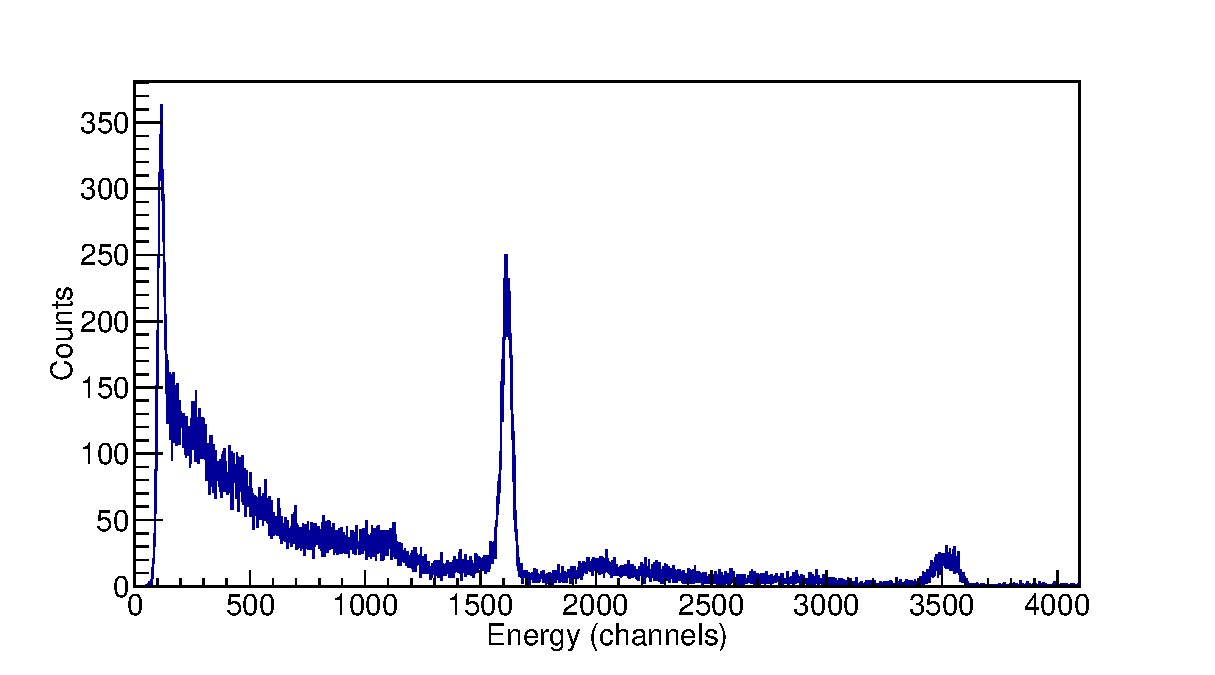
\includegraphics[width=0.80\textwidth]{labr_cs137_calibration.eps}
	\caption{LaBr\textsubscript{3}(1) response to \textsuperscript{137}Cs source.}
	\label{labr_cs137_calibration}
\end{figure}

\begin{figure}[H]
	\centering
	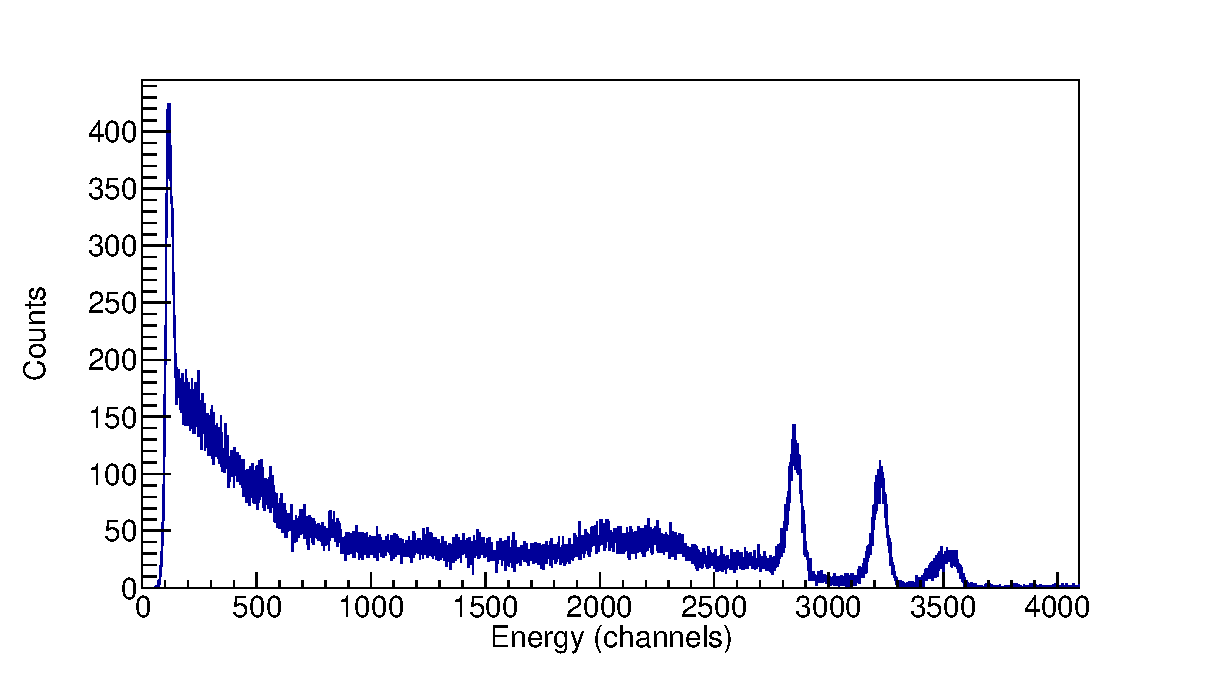
\includegraphics[width=0.80\textwidth]{labr_co60_calibration.eps}
	\caption{LaBr\textsubscript{3}(1) response to \textsuperscript{60}Co source.}
	\label{labr_co60_calibration}
\end{figure}

\subsection{The MONSTER neutron detector}
To measure the time of flight of neutrons produced by \an reactions, we use one of the modules of the MONSTER array of CIEMAT.\cite{MONSTER}
It is cylindrical, with a radius of \qty{10}{\cm} and is made out of EJ301 liquid organic scintillator.\cite{ej301}
Two smaller, liquid organic 'TADEO' scintillators were also used, but their efficiency was too low and their data too poor, hence they were not analyzed in this work.
\\

Their operating principle is the similar to that of inorganic scintillators described before, except that the excited states that emit the \textit{scintillating} light are molecular in nature, not atomic.
Organic scintillators have a higher efficiency when for detecting neutrons than inorganic ones, as neutrons excite the material mostly through $\left( \text{n},\text{p}  \right)$ reactions (unlike $\gamma$-rays), which have a higher cross-section with hydrogen atoms.

When the molecules are excited by protons instead of electrons, different states with longer half-lifes are populated and scintillating light is emmited with a higher delay.
This means that the electric pulse created by a proton is wider, which allows us to differentiate between pulses caused by detections of photons and those caused by detections of neutrons.
This is called \textit{pulse shape discrimination}, or PSD.

\begin{figure}[H]
	\centering
	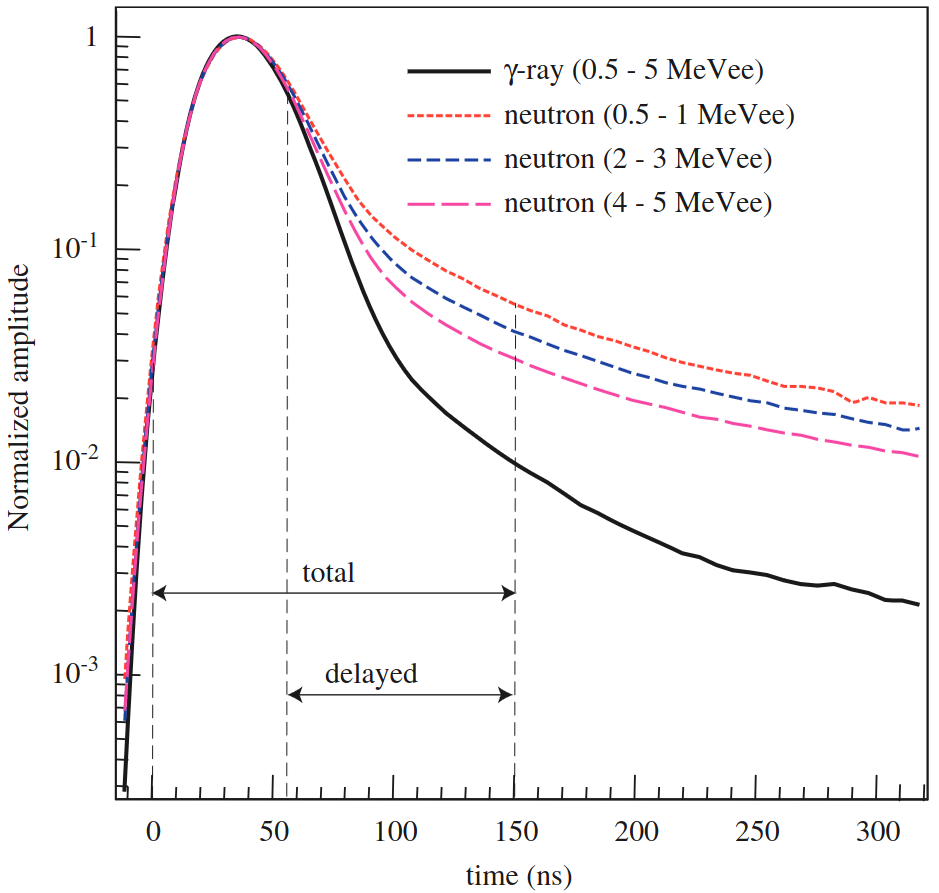
\includegraphics[width=0.65\textwidth]{psd_explanation.png}
	\caption{Scintillation pulses generated by different radiation types.
	Figure from C. Guerrero et al.\cite{guerrero2008}}
	\label{psd_explanation}
\end{figure}

By integrating the charge in a scintillation pulse in two parts, between the initial \textit{fast} rise and the latter \textit{delayed} tail, we can calculate a number, PSD:
\begin{equation}
	\text{PSD} = \frac{\text{delayed}}{\text{fast}+\text{delayed}}
\end{equation}
that we can use to separate signals corresponding to neutrons from those that correspond to $\gamma$-rays.
At high energies, the \textit{fast} portion saturates because the digitizer has limited resolution, causing the shape of the gamma tail seen in Figure \ref{example_psd}.

\begin{figure}[H]
	\centering
	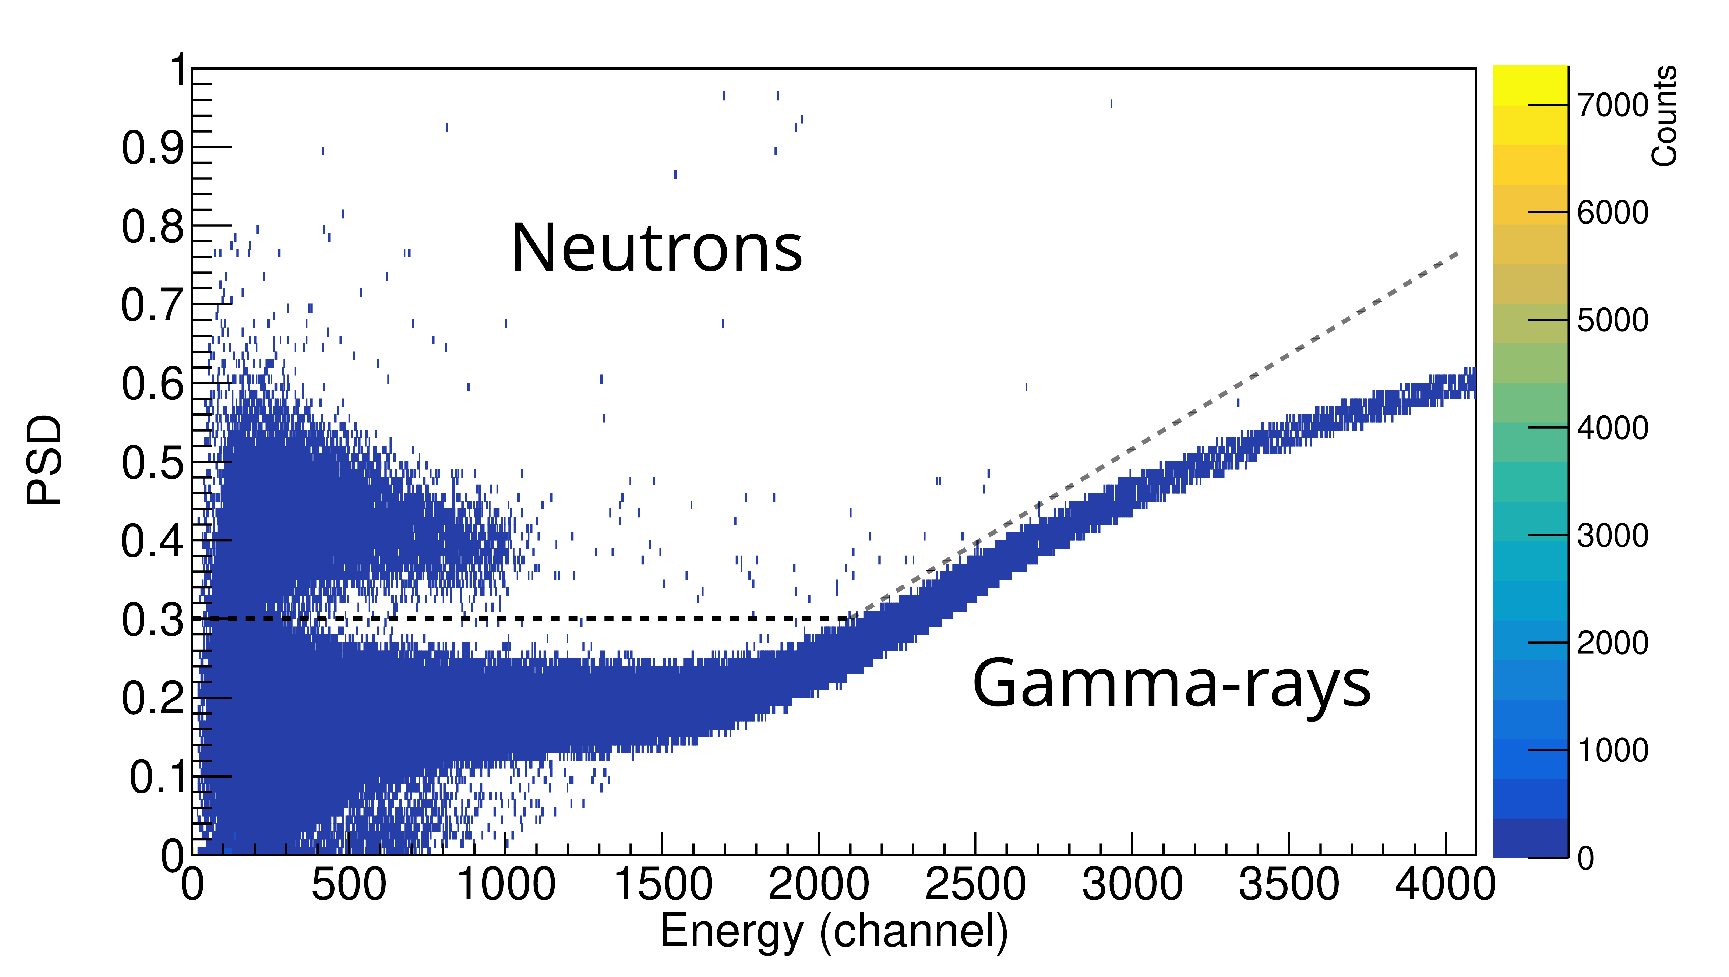
\includegraphics[width=0.80\textwidth]{example_psd.eps}
	\caption{2D histogram showing PSD separation between neutrons and $\gamma$-rays for a MONSTER measurement.
	The separation line between the two is ahown in black and dotted.}
	\label{example_psd}
\end{figure}

MONSTER's response to photons is different than the LaBr\textsubscript{3} detectors.
Because it is organic, the cross-section for the photoelectric effect is much smaller; and so photopeaks are not visible, only the Compton continuum is.

\begin{figure}[H]
	\centering
	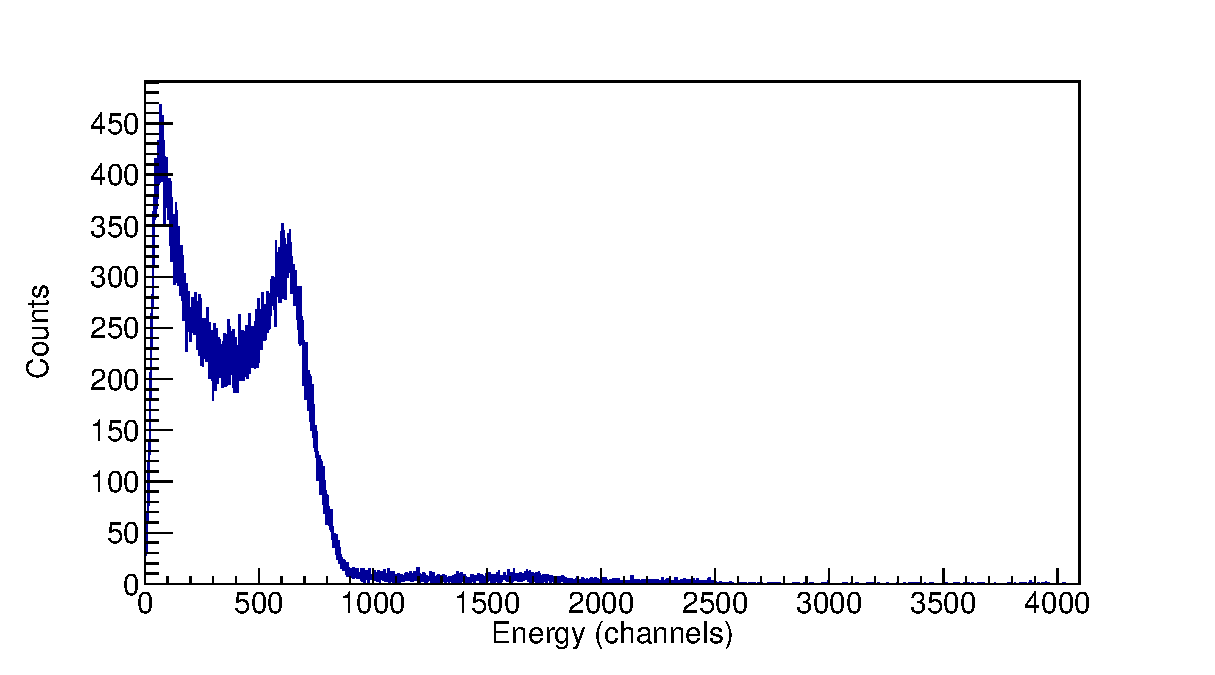
\includegraphics[width=0.80\textwidth]{monster_cs_calibration.eps}
	\caption{MONSTER response to \textsuperscript{137}Cs source.}
	\label{monster_cs_calibration}
\end{figure}

\begin{figure}[H]
	\centering
	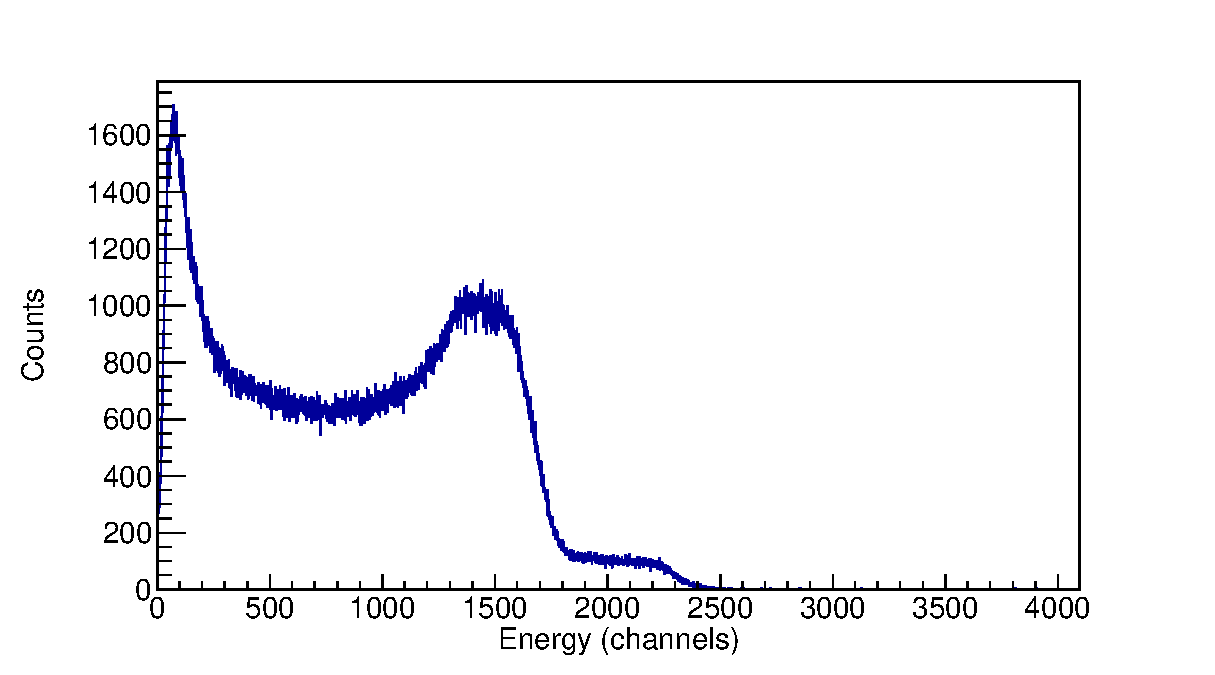
\includegraphics[width=0.80\textwidth]{monster_co_calibration.eps}
	\caption{MONSTER response to \textsuperscript{60}Co source.}
	\label{monster_co_calibration}
\end{figure}

The efficiency of the MONSTER detector to neutrons has not been calculated nor measured in this work.
Instead, it has been calculated through Monte Carlo simulations by the CIEMAT groups that owns the detector.
The efficiency curve is shown in Figure \ref{monster_efficiency}.

\begin{figure}[H]
	\centering
	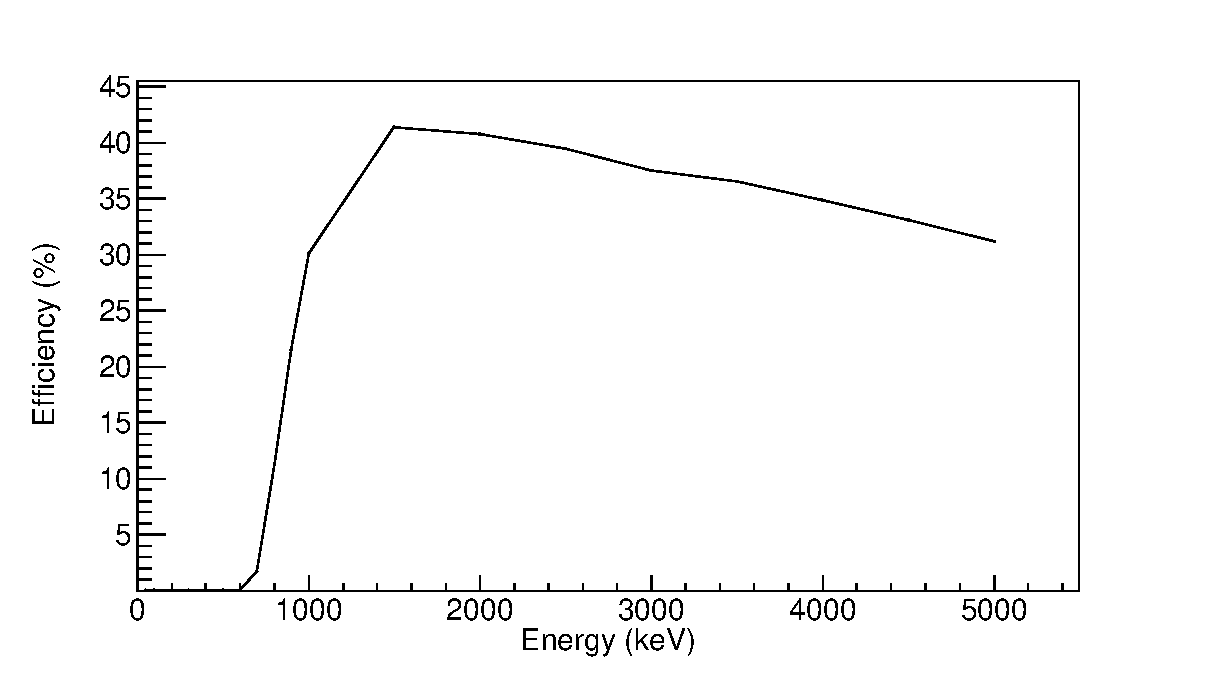
\includegraphics[width=0.80\textwidth]{monster_efficiency.eps}
	\caption{MONSTER neutron efficiency curve for an energy threshold of \qty{100}{keVee}.}
	\label{monster_efficiency}
\end{figure}

\section{DAQ}
All of the data from the detectors, as well as from the charge integrator, are connected to a \textit{data acquisition system}, or DAQ.
The one used is a CAEN 751, which has 8 channels with 10 bits resolution and sampling rate of 1 GS/s.\cite{CAEN}
It takes all of the incoming signals and saves for each one the timestamp, energy and PSD.
The data from each measurement is saved in separate ROOT files in the computer it is connected to, to be later analyzed by ROOT.\cite{ROOT}

%%%
%%%	ACTIVATION
%%%

\chapter{Neutron emission Thick Target Yield (TTY) by activation}

\section{Activation experiments}

\subsection{The activation principle}
\textit{Activation} measurements are a way of measuring the yield of a reaction in a material by measuring the decay of a resulting isotope.
For \an measurements, the beam is operated in continuous mode, launching towards the target a stream of $\alpha$ particles of a certain energy, $E_\alpha$.
When the particles hit the target, there is a certain probability \an reactions (among others) occur.
Because the target is thick enough that all $\alpha$ particles will be stopped, these reaction will take place at any $\alpha$ energy between $E_\alpha$ and, as the particles lose energy in the target, the reaction threshol of \qty{3}{\MeV}.

The number of \an reactions will be proportional to the number of incident $\alpha$ particles, and the proportionality constant is the \textbf{thick target yield}.
This is different from the regular \textit{yield}, which considers reactions at a single energy.
\begin{equation}
	\text{thick target yield} = \frac{\text{number of \an reactions}}{\text{number of incident $\alpha$ particles}}
	\label{tty_def}
\end{equation}

In \textit{activation} measurements, the number of \an reactions will be determined from the number of reaction product nuclei, by measuring their decay radiation.
For this, the reaction must produce an isotope that decays with an appropriately long half-life (not too long nor too short), and emitting radiation that we can easily detect.

Ideally, the target is to be bombarded for a period of at least a few half-lifes, and then left to decay for several more, while we measure the decay radiation.

\subsection{\Aliso\an activation at CNA HiSPANoS}
At the HiSPANoS, we have used a thick \Aliso target with \qty{95}{\percent} purity.
Each \an reaction creates a single \Piso nuclei, which is a radioactive isotope with a \qty{2.498(4)}{\minute} half-life.
We measure its $\beta +$ decay into \textsuperscript{30}Si by observing the \qty{511}{\keV} annihilation $\gamma$-rays, emmited with an intensity of \num{1.99710(8)} \cite{nucleardatasheets}.

\begin{figure}[H]
	\centering
	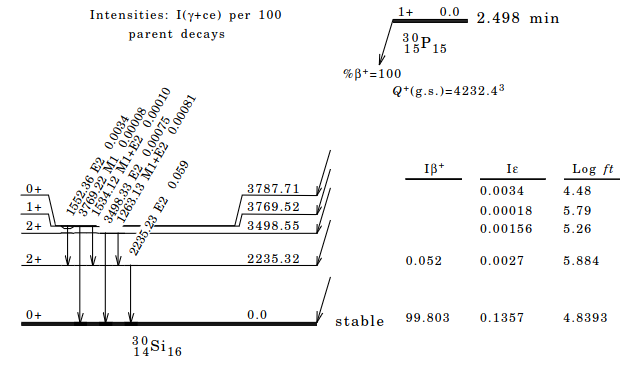
\includegraphics[width=0.7\textwidth]{Piso_decay_scheme.png}
	\caption{\Piso decay scheme.
	From \cite{nucleardatasheets}.}
	\label{Piso_decay_scheme}
\end{figure}

We irradiate the \Aliso target for several (3 to 6) half-lifes, and then let the produced \Piso decay for about 6 half-lives, so its activity becomes negligible.
During the irradiation, the number of $\alpha$ particles hitting the target is being measured by connecting a cable from the target to the current integrator, and then sent to the DAQ (setup pictured in Figure \ref{target_photo}).

\begin{figure}[H]
	\centering
	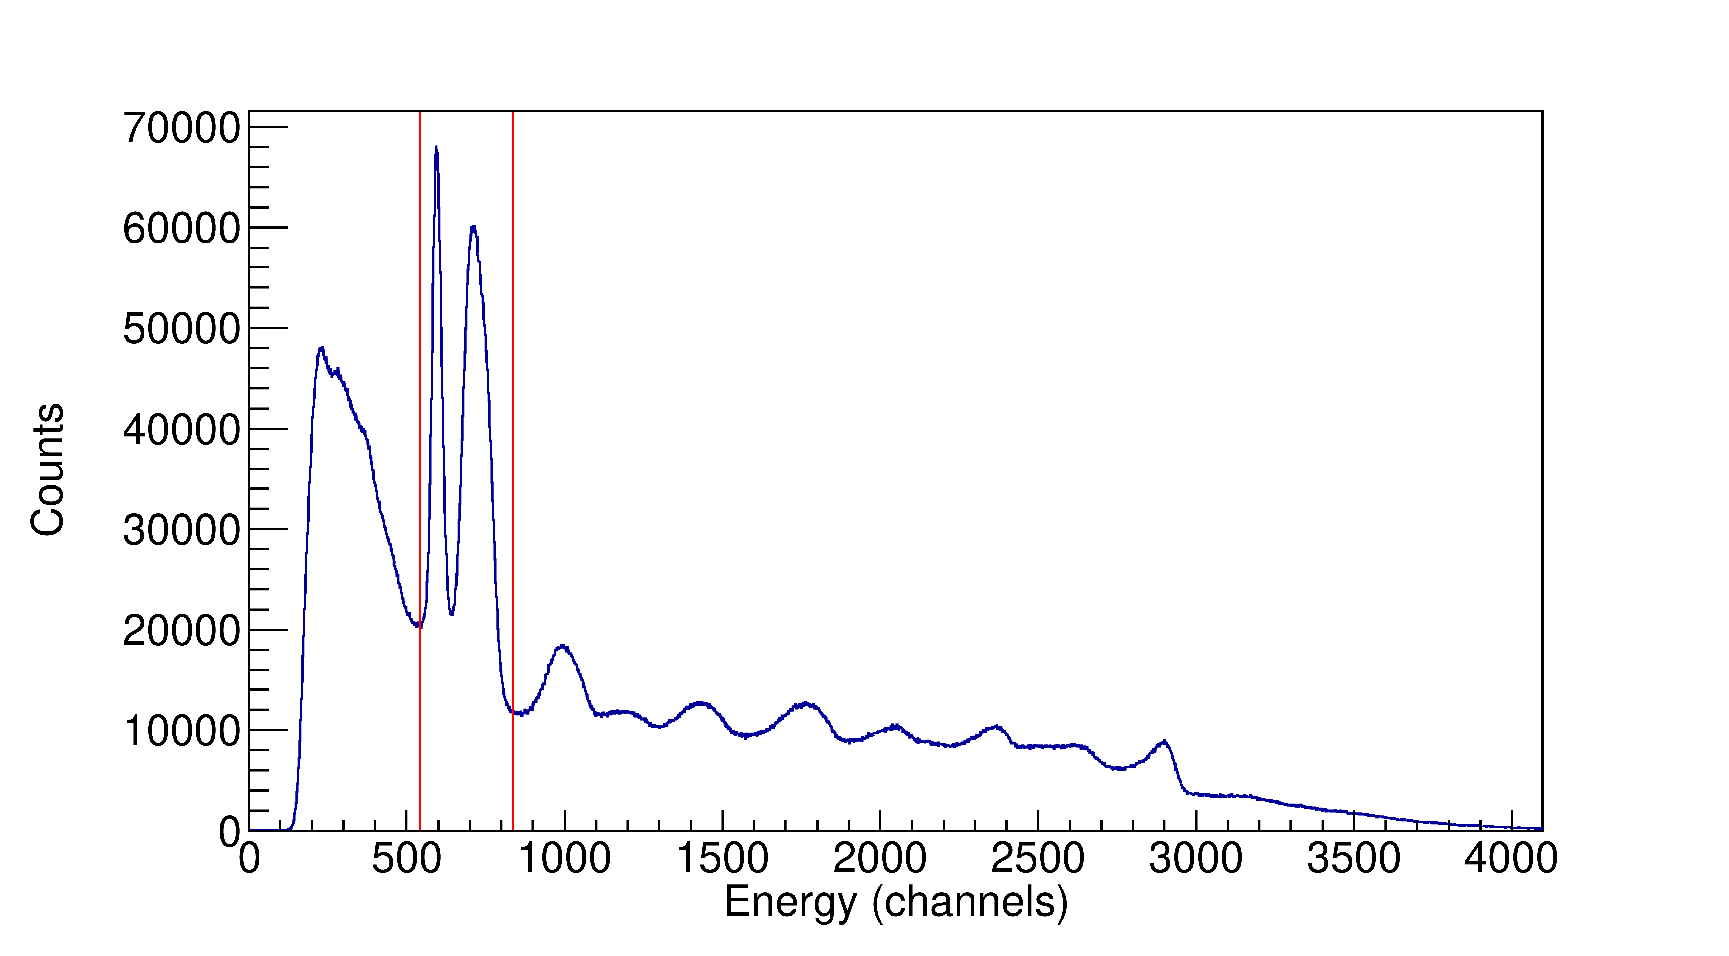
\includegraphics[width=0.80\textwidth]{example_activation_energy_histogram.eps}
	\caption{Example activation spectrum.
	The energy window used to generate the time histogram (Figure \ref{example_activation_time_histogram}) is shown in red.}	%TBD: calibrar en energía o poner "canales"
	\label{example_activation_energy_histogram}
\end{figure}

To measure the decay of \Piso nuclei, we use the two LaBr\textsubscript{3} scintillators and look at the $\gamma$-rays emitted from the target.
Figure \ref{example_activation_energy_histogram} shows the energy deposited spectrum of one of the LaBr\textsubscript{3} detectors during an activation measurement.
The reason there are two peaks, instead of the single \qty{511}{\keV} peak we would expect, is that the high rate of counts during activation affects the gain of the detectors, shifting the channel the peak corresponds to.
This is illustrated in Figure \ref{example_activation_energytime}, corresponding to an irradiation between 360 and \qty{820}{\s}.
To represent the counting rate as a function of time that allows studying the decay of \Piso, displayed in Figure \ref{example_activation_time_histogram}), we take only the counts whose energy fall inside the energy window shown in Figure \ref{example_activation_energy_histogram}.

\begin{figure}[H]
	\centering
	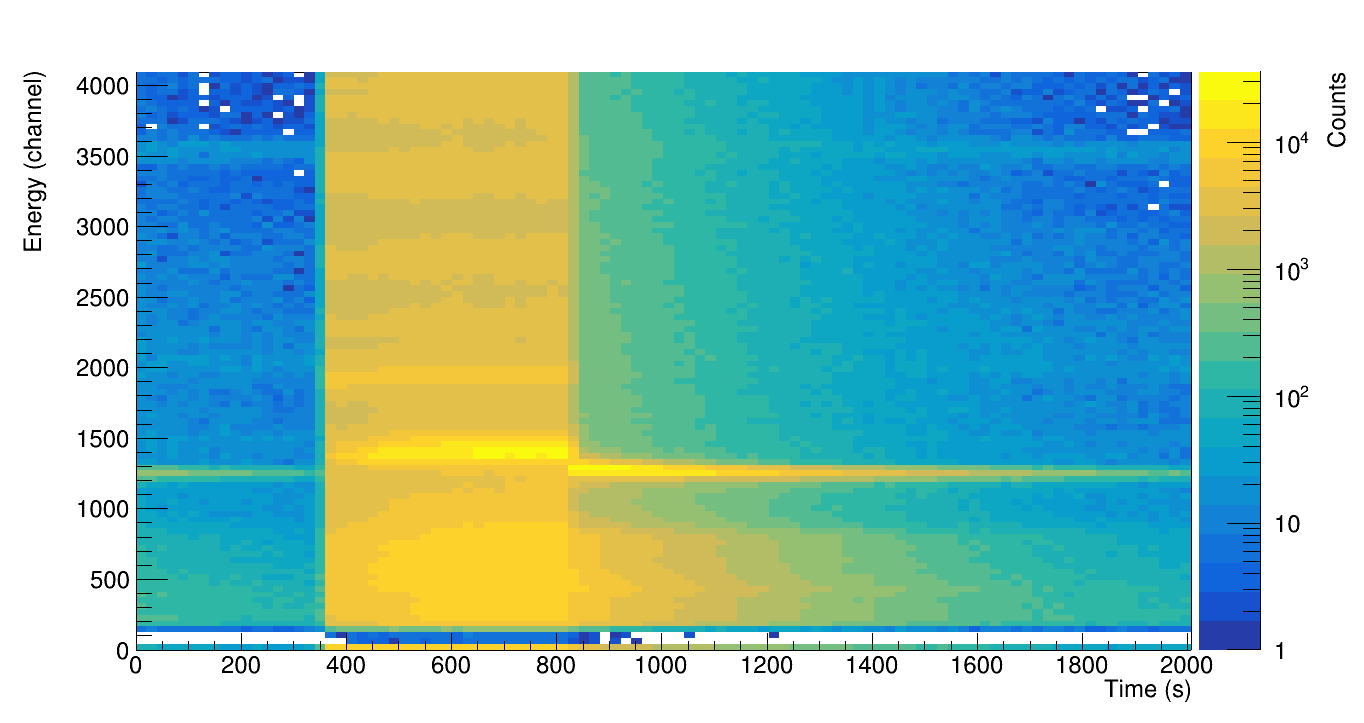
\includegraphics[width=0.80\textwidth]{example_activation_energytime.png} %TBD:eps
	\caption{Example activation spectrum over time.	%TBD: calibrar en energía o poner "canales"
	The change in energy channel for the \qty{511}{\keV} peak is labelled in black.}
	\label{example_activation_energytime}
\end{figure}

\begin{figure}[H]
	\centering
	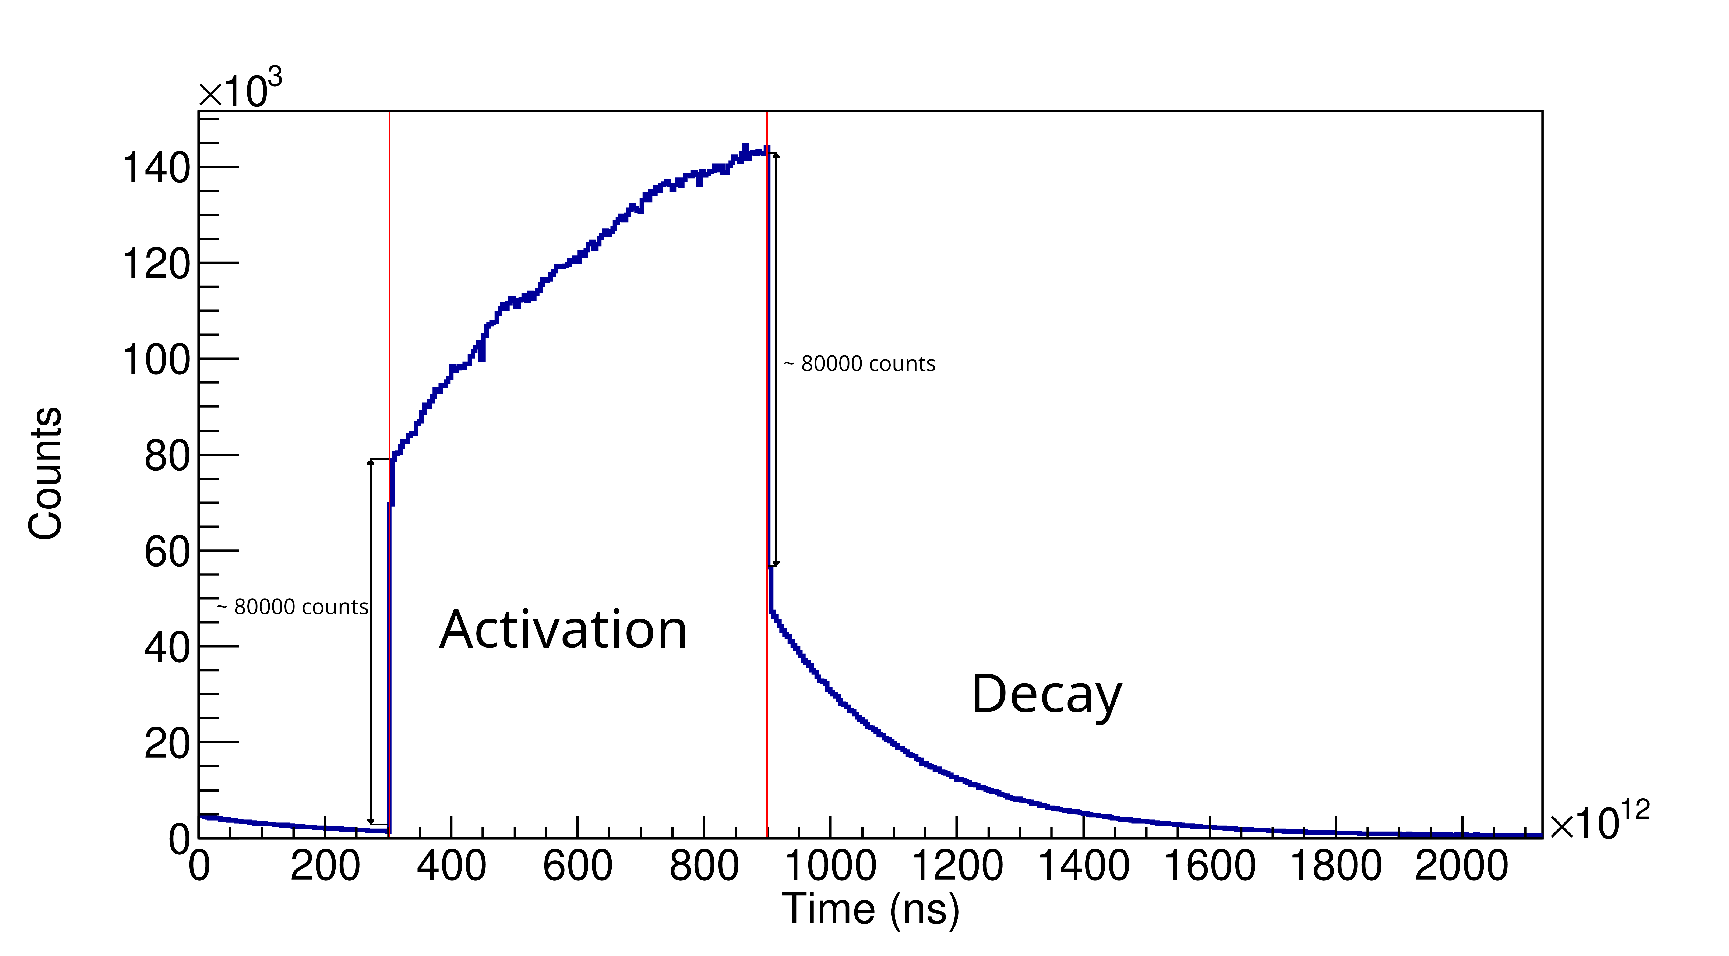
\includegraphics[width=0.80\textwidth]{example_activation_time_histogram.eps}
	\caption{Example activation time histogram.
	The activation and decay periods are labeled and separated from the rest of the histogram by red lines.
	The approximate size of the \textit{extra background} caused by the $\alpha$ particle stream is also shown.}
	\label{example_activation_time_histogram}
\end{figure}

The time distribution shown in Figure \ref{example_activation_time_histogram} shows initial counts before the activation starts, corresponding to decay of \Piso from the previous irradiation.
When the activation starts, \num{\approx 80000} counts per bin appear very quickly, going away as soon as the irradiation ends.
We call these counts the \textit{extra background}.
They are proportional to the beam current and correspond to $\gamma$-rays from \an and other reactions.

They can also be seen in Figure \ref{example_activation_energytime} as the large number of counts appearing during activation well outside of the \qty{511}{\keV} peak.
They affect the time distribution because, even if the emitted $\gamma$-rays are outside of the selected energy window, their Compton continuum may still fall inside.

After irradiation, the counts correspond to the decay of the created \Piso nuclei.

\subsection{Measurements}
The \Aliso\an activation measurements were carried out in two sessions of two consecutive days, in February and April.
Table \ref{activation_measurements_table} summarises the different measurement conditions.

Because detectors were unmounted in between both sessions, calibration measurements with \Na to determine the detector efficiency were done once for each month.

\begin{table}[H]	%Tabla con datos de las medidas de activación
\centering
\begin{tabular}[c]{>{\bfseries}r||c|c|c|c}
	N & Energy (\unit{\keV}) & Current (\unit{\nano\A}) & Activation time (\unit{\s}) & Date\tablefootnote{All took place in 2023.} \\ \hline
	1	&\num{5500}&\num{128}&\num{867}&Feb 22\textsuperscript{nd}\\ \hline
	2	&\num{7000}&\num{101}&\num{981}&Feb 22\textsuperscript{nd}\\ \hline
	3	&\num{8500}&\num{128}&\num{909}&Feb 22\textsuperscript{nd}\\ \hline
	4	&\num{8500}&\num{192}&\num{899}&Feb 23\textsuperscript{rd}\\ \hline
%	5	&\num{5500}&\num{123}&\num{605}&Apr 17\textsuperscript{th}\\ \hline
%	6	&\num{5500}&\num{312}&\num{599}&Apr 17\textsuperscript{th}\\ \hline
	5	&\num{8250}&\num{193}&\num{452}&Apr 18\textsuperscript{th}\\ \hline%7
	6	&\num{7000}&\num{216}&\num{466}&Apr 18\textsuperscript{th}\\ \hline%8
	7	&\num{5500}&\num{151}&\num{451}&Apr 18\textsuperscript{th}\\ \hline%9
	8	&\num{7500}&\num{183}&\num{448}&Apr 18\textsuperscript{th}\\ \hline%10
\end{tabular}
\caption{Activation measurements}
\label{activation_measurements_table}
\end{table}

\section{Data analysis}
We can determine the activity from \Piso nuclei in the target using the differential equation:
\begin{equation}
	\ddt{N(t)} = P(t) -\lambda N(t) = P(t) - A(t)
	\label{activation_diffeq}
\end{equation}
where $\lambda$ is the decay constant of \Piso, $N(t)$ is the number of \Piso at time $t$, $P(t)$ is the \Piso production of \Piso (number of \Piso nuclei produced by \an reactions per unit of time) and $A(t)$ is the activity.
The Thick Target Yield of the reaction (TTY) can then be calculated from the production and the beam current:
\begin{equation}
	\text{TTY} = \frac{P(t)}{I_\alpha(t)}
	\label{TTYfromP}
\end{equation}
\\

Our goal being to get the thick target yield from $P(t)$, what we will actually analyze is the activity of \Piso nuclei as they decay by $\beta +$, which will be $A(t) = \lambda N(t)$.
In order to do that, we use the two LaBr\textsubscript{3} scintillators to detect \qty{511}{\keV} $\gamma$-rays.
Some counts will be background, corresponding not to \Piso decays, but to the Compton continuum of higher energy emissions either in the environment or due to other reactions caused by the $\alpha$ particles in the target.
In order to get the activity in decays per second, we must subtract the background $b(t)$ from the \qty{511}{\keV} counts $c(t)$ shown and then divide by the intensity of the emission ($I_{511}=\num{1.99}$), the histogram bin width ($b_{\Delta t}$) and the detection efficiency ($\varepsilon_{511}$):
\begin{equation}
	A(t) = \frac{c(t) - b(t)}{I_{511} b_{\Delta t} \varepsilon_{511}}
	\label{ctoA}
\end{equation}

In order to get the TTY using \ref{TTYfromP}, we need to determine $P(t)$.
We use two different methods to get $P(t)$ from $A(t)$, depending on the part of the time interval being looked at.

\subsection{Analysis of the decay curve}
After the irradiation is over, we are left with a certain number of \Piso nuclei that will decay following a radioactive decay law.
For the \textit{decay} fit, we simply fit this part of the time histogram to a negative exponential plus a constant background, $A(t) = A\textsubscript{EOA} e^{-\lambda t} + B$ to get the \Piso activity at the end of activation, $A$\textsubscript{EOA}.
Instead of converting counts to activity using \ref{ctoA}, which woud require us to know the background beforehand, we actually fit the counts directly to $c(t) = c\textsubscript{EOA} e^{-\lambda t} + B$ and later convert the result of the fit, $c\textsubscript{EOA}$ by doing:
\begin{equation}
	A\textsubscript{EOA} = \frac{c\textsubscript{EOA}}{I_{511} b_{\Delta t} \varepsilon_{511}}
\end{equation}

The fit is implemented using the ROOT \textit{fit} method, with $c$\textsubscript{EOA}, $\lambda$ and $B$ as fit parameters.
The value of the decay constant $\lambda$ is fixed to that of \Piso, and not determined by the fit.
However, it can be left free so that ROOT calculates its value, both to make sure that no other isotope is being produced at significant quantities, and as a sanity check.
Because that test was successful, the parameter is fixed to the known value of $\lambda$ and following fits only return two values: $c$\textsubscript{EOA} and $B$.
\\

We then divide $A$\textsubscript{EOA} by $\lambda$ to get the number of \Piso nuclei at the end of activation, $N$\textsubscript{EOA}.
However $N$\textsubscript{EOA} is not all of the \Piso nuclei created by \an reactions, as some will have decayed during the activation period:
\[ \frac{A_\text{EOA}}{\lambda} = N_\text{EOA} \neq \int_{\Delta t}P(t) \dif t \]

\begin{figure}[H]
	\centering
	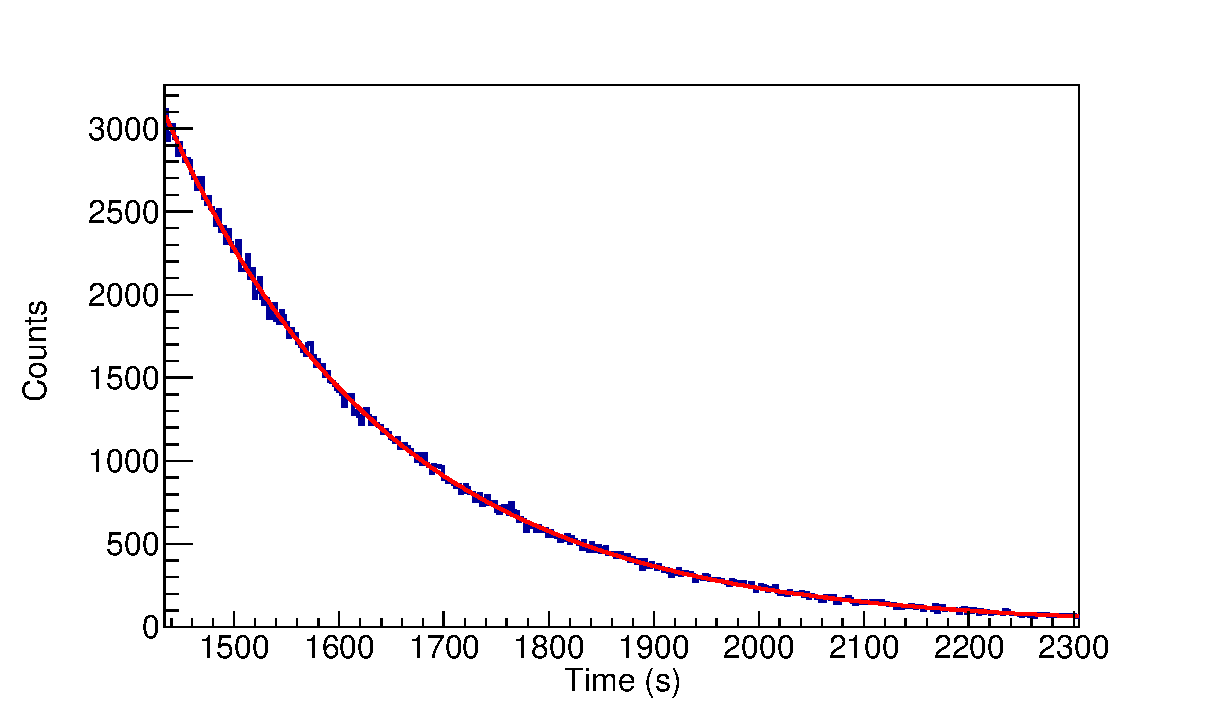
\includegraphics[width=0.80\textwidth]{example_decay_fit.eps}
	\caption{Example decay fit (red) to the data (blue).}
	\label{example_decay_fit}
\end{figure}

We can solve the differential equation \ref{activation_diffeq} during the activation period analytically by taking $P(t)$ as a constant, $P$:
\begin{equation}
	\ddt{N} = P -\lambda N
\end{equation}
its solution being:
\begin{equation}
	N(t) = \frac{P}{\lambda} + \left(  N_0 - \frac{P}{\lambda}  \right) e^{-\lambda t}
	\label{activation_constantP_solution}
\end{equation}
with $N_0$ the initial number of \Piso nuclei, assumed to be \num{0}.
After a long irradiation ($t>>t_{1/2}$), $N(t)\longrightarrow P/\lambda$, meaning that the production rate equals the decay rate.
This effect is called \textit{saturation}, and means that, for long enough activations, one can simply take $A_\text{EOA}\approx P$.

If that approximation cannot be made (which is our case), then:
\[ N\textsubscript{EOA} =N(\Delta t) = \frac{P}{\lambda} \left(1 - e^{-\lambda \Delta t} \right)\Longrightarrow A\textsubscript{EOA}=P\left(1-e^{-\lambda\Delta t}\right)\Longrightarrow \]
\begin{equation}
	P = \frac{A\textsubscript{EOA}}{1 - e^{-\lambda \Delta t}}
\end{equation}
with $\Delta t$ the irradiation time.
Then, $P\cdot\Delta t$ is the total number of \Piso nuclei created during the activation, meaning we can now get the Thick Target Yield, according to equation \ref{TTYfromP}, as:
\begin{equation}
	\text{TTY} = \frac{P}{I_\alpha} = \frac{A_\text{EOA}}{I_\alpha \left( 1-e^{-\lambda \Delta t}  \right)} =
	\frac{c_\text{EOA}}{I_\alpha \left( 1-e^{-\lambda \Delta t}  \right) I_{511} b_{\Delta t} \varepsilon_{511}  }
\end{equation}
where $c_\text{EOA}$ is obtained directly as the result of the fitting, and the current $I_\alpha$ we obtain from the current integrator, by dividing the total number of $\alpha$ particles over $\Delta t$.
\\

The advantages of this method are over the one presented in the next section are:
\begin{itemize}
	\item The fitting is simple and fast.
	\item Only the total number of incident $\alpha$ particles is needed, not information of current over time.
	\item The \textit{extra background} doesn't bother us, as we only care about the counts once activation ends.
	\item It is the standard way to carry out activation measurements.
\end{itemize}
The main disadvantage is that, because it assumes $P(t)$ to be constant, the method won't work if the $\alpha$ particle current $I_\alpha$ is not approximately constant over time.

\subsection{Analysis of the production and decay curves simultaneously}
Instead of taking $P(t)$ as constant and integrating \ref{activation_diffeq} analytically, another option is to fit the whole histogram to a function that numerically integrates equation \ref{activation_diffeq} step by step.
We call this fit the \textit{unified} fit.

The function takes the data of beam current over time as input, and calculates $P(t)$ every step as $P(t) = \text{TTY}\cdot N_\alpha$, with $N_\alpha(t)$ the number of incident $\alpha$ particles during the step.
This is particularly useful because the current is not perfectly constant, there are drops and rises in many of the measurements (Figure \ref{current_histograms}) and this could make the \textit{decay} fit (previous section) less precise, as the assumption of constant current could be incorrect.
\\
\begin{figure}[H]
	\centering
	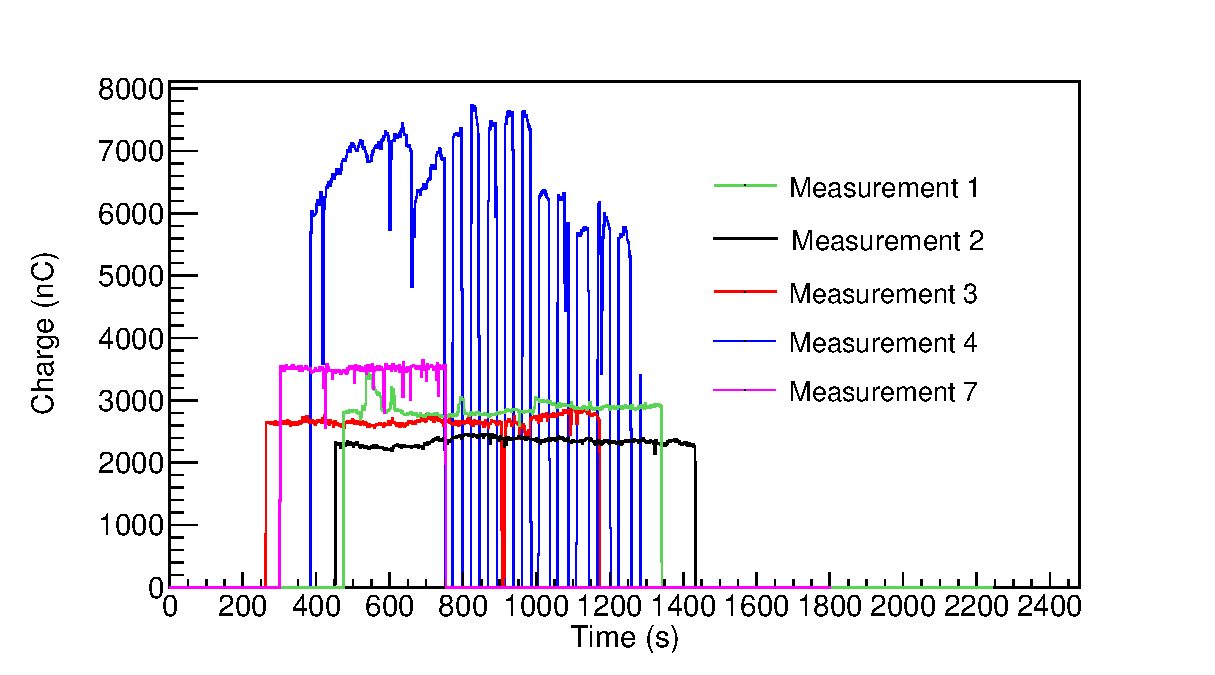
\includegraphics[width=0.80\textwidth]{current_histograms.eps}
	\caption{All current histograms, superimposed.
	Most different in number 4, which has periodic losses of information due to a failure of the DAQ.
	Although current data is lost, the total charge was still recorded.}
	\label{current_histograms}
\end{figure}

The function is implemented using a C++ functor, and the fitting using ROOT's \textit{fit} method.
Every step, it calculates $P(t) = \text{TTY}\cdot N_\alpha(t)$, then assumes $P$ constant for the duration of the step.
It then sets the new number of \Piso nuclei as:
\begin{equation}
	N(t+\dif t)=\frac{P(t)}{\lambda} + \left( N(t)-\frac{P(t)}{\lambda} \right) e^{-\lambda \dif t}
\end{equation}
then repeats until the end of the data.
This integrates equation \ref{activation_diffeq} numerically, using the analytical solution \ref{activation_constantP_solution}.

The function needs to output the counts over time $c(t)$ every step calculating it from $N(t)$, so that ROOT can compare it to the histogram of \qty{511}{\keV} counts over time for fitting.
To that end, we make the function return:
\[ c(t) = A(t)I_{511}b_{\Delta t}\varepsilon_{511} - B = \lambda N(t) I_{511}b_{\Delta t}\varepsilon_{511} - B\]
where $B$ is a constant background that the function also fits.
The function also considers an initial number of \Piso (from previous activation runs) and a number of counts proportional to the current (by adding that to $c(t)$), which correspond to the \textit{extra background}.
All of those are also parameters for the fitting, and also adjusted by ROOT.

The TTY is one of the parameters adjusted by the fitting (it is used to calculate $P(t)$), and so it is outputted by ROOT directly when the function is fitted, in units of \an per $\alpha$.
\\

\begin{figure}[H]
	\centering
	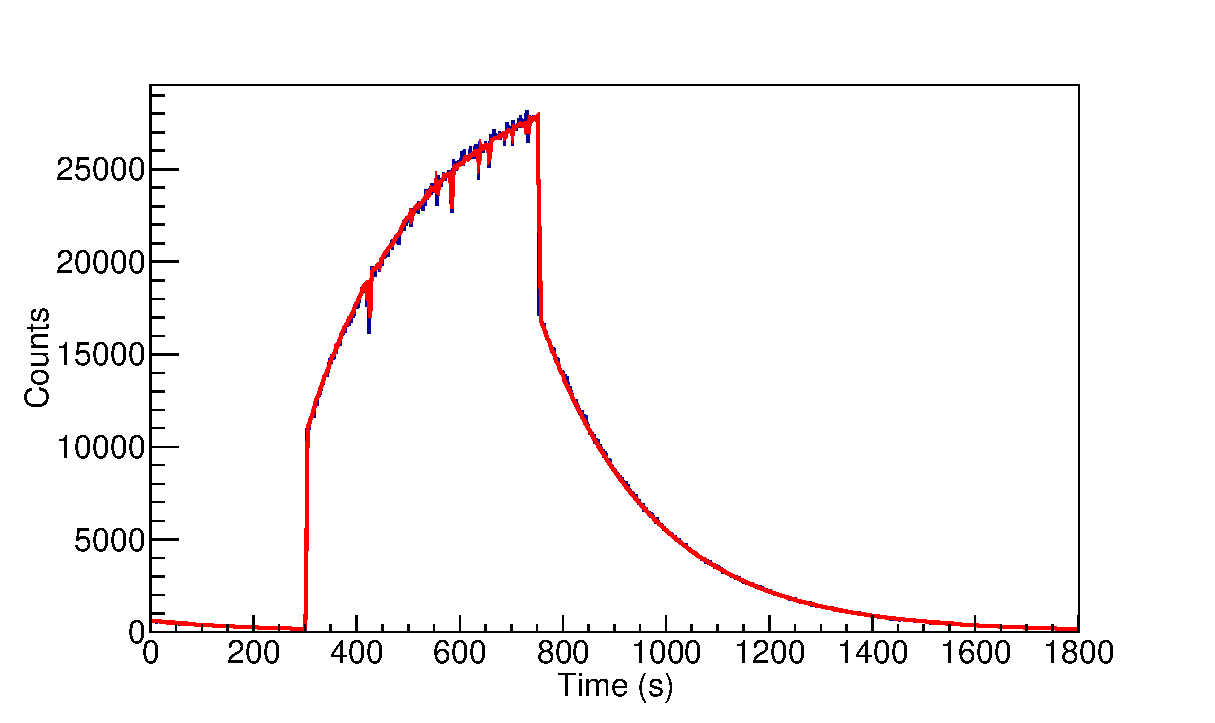
\includegraphics[width=0.80\textwidth]{example_unified_fit.eps}
	\caption{Example unified fit (red) and data (blue).}
	\label{example_unified_fit}
\end{figure}

Figure \ref{example_unified_fit} show the fit (red) to the counts (blue).
We can see that it adjusts very well to the data.
In Figure \ref{example_unified_fit}, we can see that it also correctly accounts for an initial amount of \Piso from a previous activation, as well as the \textit{rise} and \textit{decay} periods.
\\

Data of current over time was not recorded in half of the measurements in April (numbers 6, 7 and 8) because the current measuring cable was, by mistake, not connected to the DAQ.
In addition, measurement number 4, in February, shows loss of data during the irradiation due to a problem with the DAQ.
These issues prevent the \textit{unified} fit from being used for all measurements.

\begin{figure}[H]
	\centering
	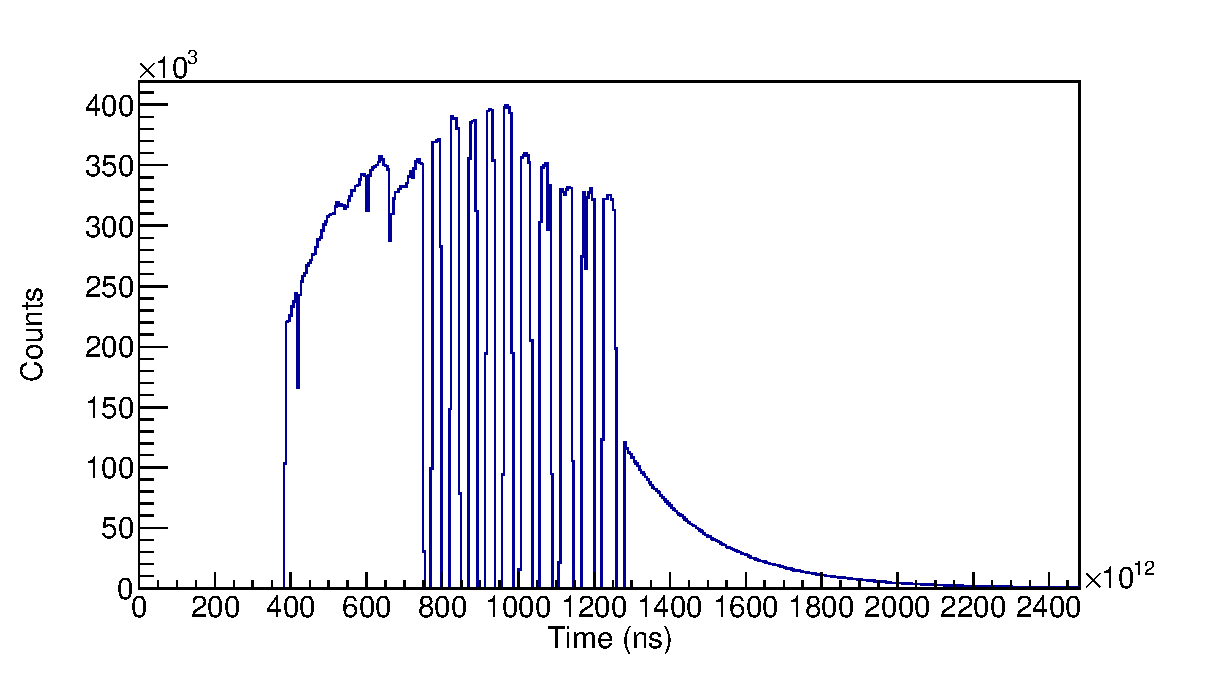
\includegraphics[width=0.80\textwidth]{activation_4_time.eps}
	\caption{Activation measurement number 4.
	We can see the loss of signal to the DAQ periodically for most of the activation period.}
	\label{activation_4_time}
\end{figure}

\section{Results}
Because all measurements were carried out with two detectors, we can start by comparing them.
Afterwards, we can compare the different methods with each other, to find out whether they agree.
These comparison will give some information about the systematic uncertainty of the results.
Then, we can compare our results with the literature published in the EXFOR database.\cite{jacobs}

\subsection{Comparison between detectors}
In principle, both detectors should give the exact same result.
However, Figure \ref{decay_errors_rel_per} shows that the relative difference in measurements between LaBr\textsubscript{3} detectors 1 and 2 is around \qty{4}{\percent} in February and \qty{8}{\percent} in April.
The points shown are for \textit{decay} fit measurements only (for the sake of brevity), but are similar for the other methods.
In the following sections, the values shown correspond to the mean between the two detectors, with an uncertainty equal to half of the difference between them.

Measurements in February show negative values, indicating detector 2 is higher; while those in April are positive, meaning the opposite is true.
\\

\begin{figure}[H]
	\centering
	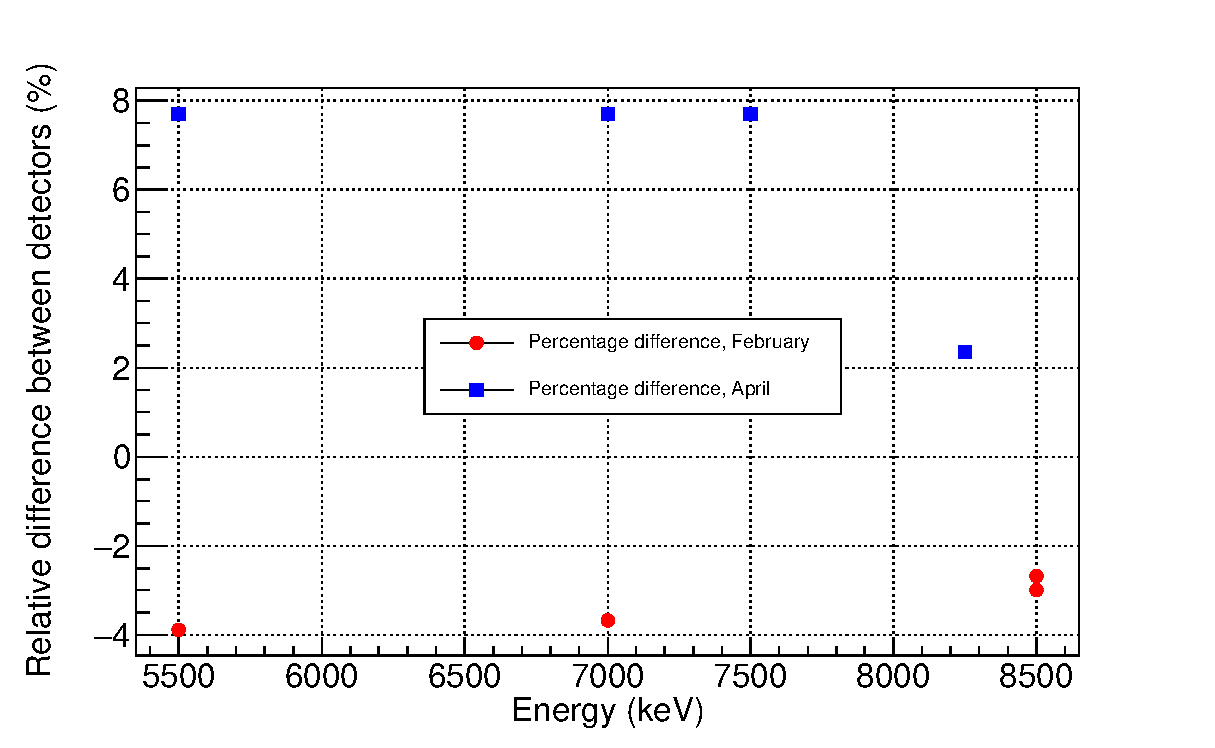
\includegraphics[width=0.80\textwidth]{decay_errors_rel_per_fixed.eps}	%TBD:poner eje y de -10 a 10
	\caption{Percentage difference in thick target yield results between detectors in each measurement.
	The number shown is calculated as $\frac{\text{LaBr}_1-\text{LaBr}_2}{\text{LaBr}_1+\text{LaBr}_2}\cdot 100$: half the difference, over the average, in percentage.}
	\label{decay_errors_rel_per_fixed}
\end{figure}

The best agreements between detectors are for the measurements at higher energies, in both months.
The differences barely changing at energies under \qty{8}{\MeV}, and we can see at \qty{8.5}{\MeV}, where we have two measurements, that they give very similar numbers.
All of this tells us that this difference is due to a systemic error, and that it is likely dependent on the energy of the accelerator.

Regardless, agreement between detectors is reasonable and consistent, and going forward we will represent, for each measurement and method, the average between both detectors.

\subsection{Comparison between analysis (\textit{decay} vs. \textit{unified}) methods}
To determine the agreement between the different fit methods, we can calculate the relative difference between the results given by each, as in the previous section.
\\

In Figure \ref{activation_method_comparison} are represented the relative difference when comparing the \textit{unified} and \textit{decay} methods.
Because we don't have current data (and thus \textit{unified} results) for mesurements 4, 6, 7, and 8; we only have 4 measurements to do this comparison with.
Luckily, they are each at a different alpha energy and so the study is complete.

\begin{figure}[H]
	\centering
	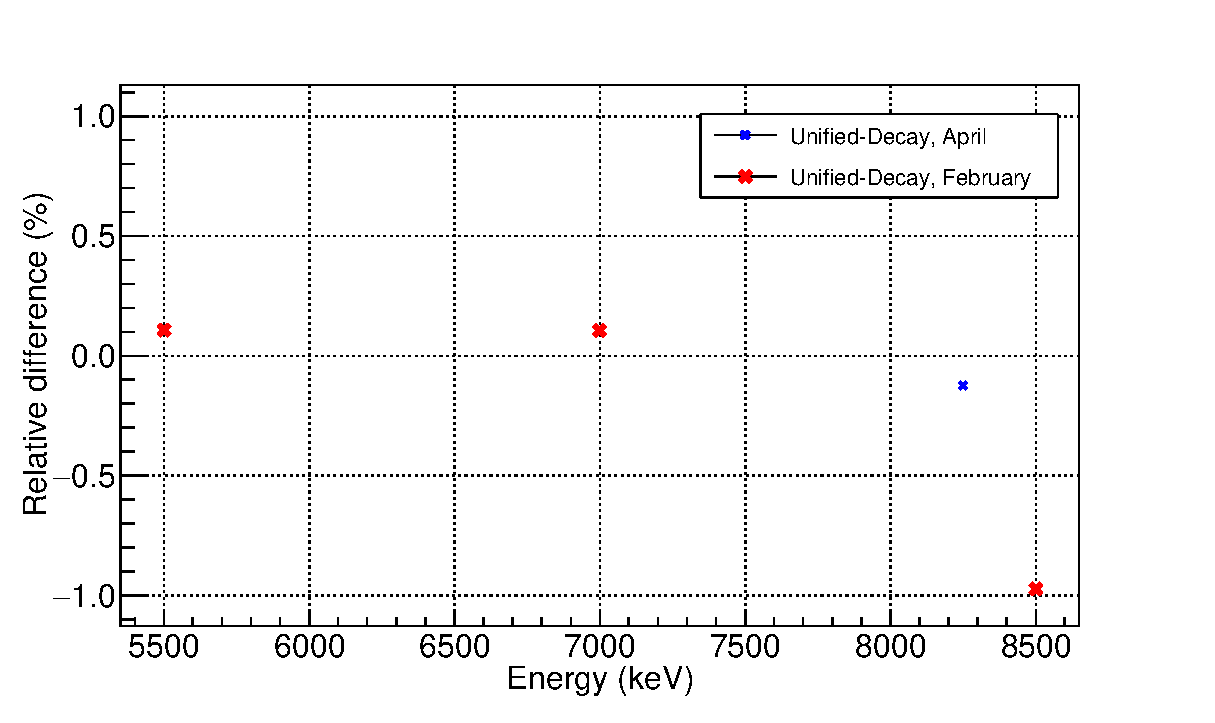
\includegraphics[width=0.80\textwidth]{activation_method_comparison.eps}	%TBD:dejar solo decay y unified y poner eje y de 2 a -2
	\caption{Relative difference between the different fitting methods, with different symbols for each comparison; and color for each month.}
	\label{activation_method_comparison}
\end{figure}

We can see that the agreement is better than \qty{1}{\percent} between \textit{unified} and \textit{decay} fit methods, for all measurements.
This means that the discontinuities in the beam delivery during the irradiation and slight changes in the beam intensity are not significant enough to prevent using the very simple \textit{decay} fit method.
This is excellent news because, unfortunately, as mentioned before we don't have beam current data for measurements 4, 6, 7, and 8.

In the following, all the data shown correspond to the decay fit results.
\\

\subsection{Comparison with data from the literature}
The Thick Target Yield (TTY) obtained experimentally in this work have been compared with the results from G. J. H. Jacobs and H. Liskien\cite{jacobs}, extracted from the EXFOR database.
In figure \ref{activation_final_results} we show this comparison, evidencing that the disagreement is very large, nearly a factor of \num{2}.
The agreement becomes really good when scaling the EXFOR data by 1.9, which is the upper curve shown in the same figure.

\begin{figure}[H]
	\centering
	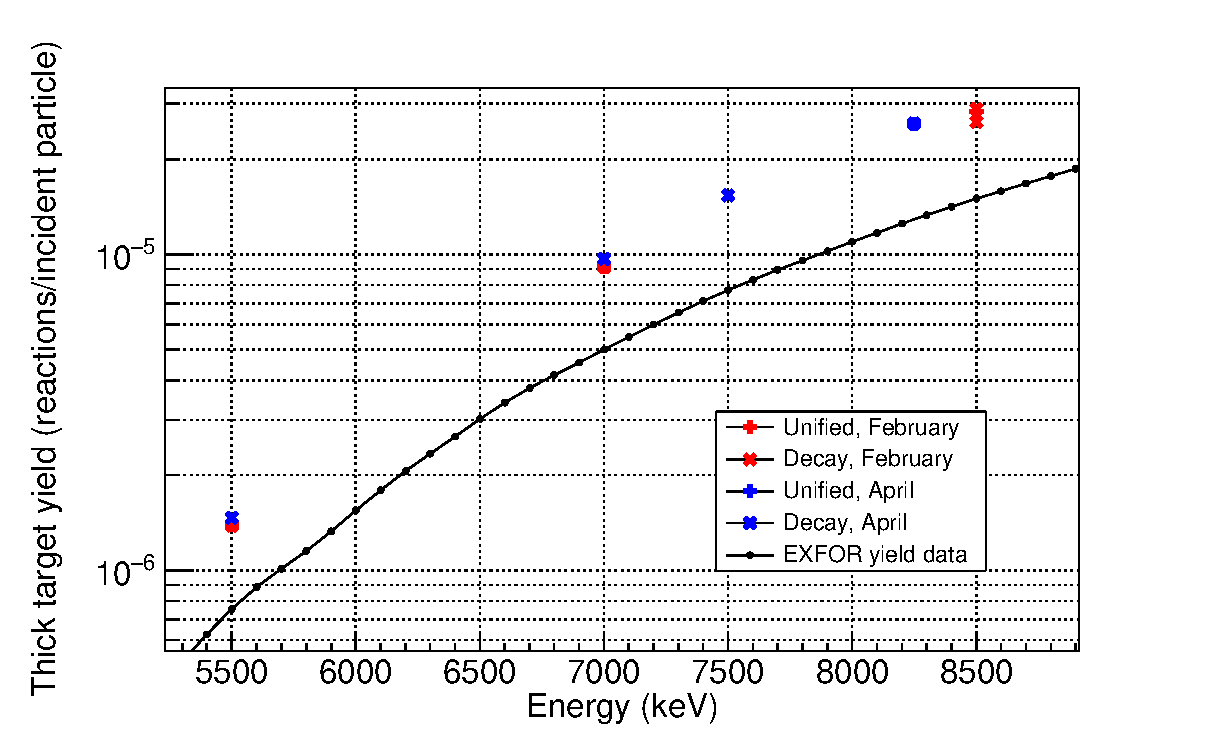
\includegraphics[width=0.80\textwidth]{activation_final_results.eps}	%TBD:añadir nombre de referencia en leyenda, y neutrons/alpha en el eje y
	\caption{Final results for thick target yield, next to the data from G. J. H. Jacobs and H. Liskien\cite{jacobs} and a scaled up version.}	%TBD:poner referencia
	\label{activation_final_results}
\end{figure}

Figure \ref{activation_result_diffs} shows the ratio of results from this work over G. J. H. Jacobs and H. Liskien.\cite{jacobs}
The mean difference and the standard deviation between all measurements is \num{1.90(9)}, which means that the energy dependence of the TTY is reproduced within \qty{5}{\percent}, which is very good considering that the level of agreement between the two detectors is of the same order.
Looking carefully at the dates of the experiments, the ratio in February is \num{1.84(6)} while that of April is \num{1.98(3)}.
This \qty{7}{\percent} difference should only be related by the fact that the measurements took place in different period and hence the accelerator and detection set-up may have an influence up to about that level in the results.
This should be to be studied further.

\begin{figure}[H]
	\centering
	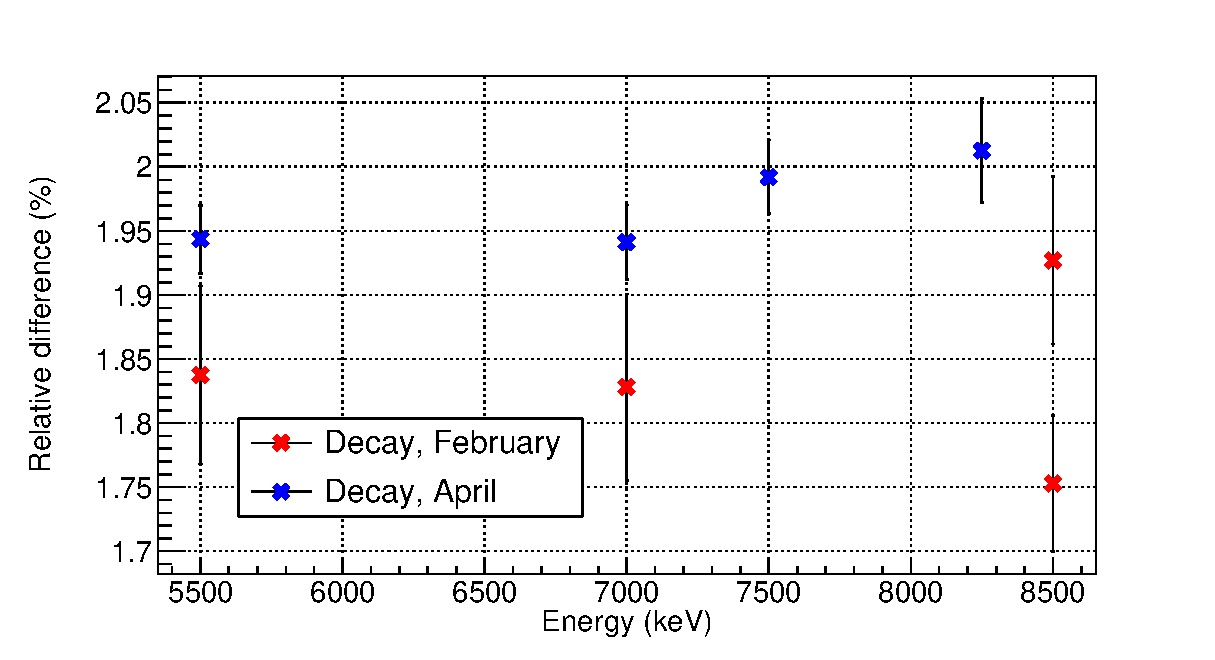
\includegraphics[width=0.80\textwidth]{activation_result_diffs.eps}	%TBD: cambiar eje y a TTY (This work/G. J. H. Jacobs and H. Liskien)
	\caption{Ratio of TTY values from this work and from G. J. H. Jacobs and H. Liskien\cite{jacobs} as a function of the beam energy.}	%TBD:añadir nombre referencia
	\label{activation_result_diffs}
\end{figure}

In conclusion, although the activation measurements are consistent with each other and the resulting shape is consistent with the data from the literature; the absolute value is too high, by a factor of \num{1.90(9)}.
This is most likely due to an unidentified error in the data analysis, whose cause remains a mystery.
The error must necessarily, affect all fit methods employed and all measurements, as the have all been found to be compatible.


%%%
%%%	TOF
%%%

\chapter{Measuring neutron energy by time-of-flight}

\section{The time-of-flight experiments}
The most accurate, and sometimes the only, method for determining the kinetic energy energy of a neutron is by time-of-flight.

\subsection{The time-of-flight principle} 
This method requires that the beam of particles producing the neutrons features a pulsed beam structure: the $\alpha$ particles should arrive in narrow pulses spaced with a certain period, producing as a results neutrons also in the form of pulses.
\\

The time that the radiation needs to reach the detector since it is produced is called the \textit{time-of-flight}, or ToF.
In the case of $\gamma$-rays, they move at the speed of light $c$, and thus all arrive at the detector at $\text{ToF}=L/c$, with $L$ the distance to the target, forming the so-called  \textit{gamma flash}.
Neutrons, however, have different speeds depending on their kinetic energy and therefore arrive at the detector with a ToF distribution from which the neutron energy distribution produced by the \an reaction can be extracted.
For each neutron:
\begin{equation}
	E_n=\frac{1}{2} m_n \left( \frac{L}{\text{ToF}} \right)^2 = \frac{1}{2} m_n \left( \frac{L}{t_n - t_{flash} + L/c} \right)^2
	\label{Eq_ToF2En}
\end{equation}
where $L$ is the distance between the target and the detector, and where the ToF of the neutrons is calculated in reference to the time of the $\gamma$-flash $t_{flash}$ and of the neutron $t_n$ in reference to some other point in time.

The neutron energy resolution that can be achieved can be calculated through propagation of errors as:
\begin{equation}
    \frac{\Delta E_n}{E_n} =
    2\sqrt{\frac{c^6\left(t_n-t_\text{flash}\right)^2\left(t_n-t_\text{flash}+\frac{L}{c}\right)^4}{\left(c\left(t_n+t_\text{flash}\right)+L\right)^6}\left(\frac{\Delta L}{L}\right)^2 + \frac{\Delta t_n^2 + \Delta t_\text{flash}^2}{{\left(\frac{L}{c}+t_n-t_\text{flash}\right)}^2}}
    \label{Eq_Enresolution}
\end{equation}

Hence, the resolution is better as the detector is placed further from the target (approximately, $\Delta E_n/E_n \propto L^{-2}$) and as the beam pulses become narrower (as this is it what causes  $\Delta$t$_{flash}$, the fact the $\alpha$ particles do not arrive all at the same time).
The beam pulses always have a certain width that generally can be approximated by a Gaussian distribution.

In order to study the time structure of the beam pulse, the shape of the observed $\gamma$-flash is a good proxy, because the photons travel all at the same speed and are directly caused by the $\alpha$ particles in the beam.
The gamma-flash will thus have the same shape as the alpha pulse, simply scaled by a factor and with an added background from other sources.

\subsection{Time-of-flight implementation at HiSPANoS} 
In order to measure the ToF distribution, each time the accelerator's chopper acts, its internal clock emits an electric signal that is sent through a long cable to the DAQ, which takes it as a reference signal, from wich to determine $t_{flash}$ and $t_n$.
It doesn't correspond to when the pulse arrives at the target, as the time the particles take to cover the distance is not the same as the time taken by the electric signal to travel along the cable and be registered.

The detector signals from photons and neutrons are registered and marked with the timestamp relative to the chopper clock.
The result is a ToF distribution of signals that, in order to have physical meaning, need just to be shifted so that the $\gamma$-flash falls in the $\text{ToF}=L/c$ position.
\\

An example of the observed $\gamma$-flash is displayed in Figure \ref{example_gflash}.	%YO ENSEñARÍA SOLO UNA PARA PODER DESCRIBIRLA BIEN, Y LUEGO TODAS EN LA SIGUIENTE SECCION PARA DISCUTIR LA CASUÍSTICA
The time structure of the $\gamma$-flash is far from the ideal Dirac delta function.
First, it features a quasi-Gaussian profile with a FWHM of \qty{1.5}{\nano\second}, which will certainly affect the neutron energy resolution (see equation \ref{Eq_Enresolution}).
Then, it also features a tail with a bump at longer ToF values, and a constant background.
This is related to the fact that the buncher is optimized for protons and deuterons, but not for $\alpha$ particles.

In the worst case (measurement 1), the tail contains up to \qty{30}{\percent} of the overall $\gamma$-flash, which means that the time of arrival of the alpha beam is not very well determined.
Because of all this, we cannot really treat the $\gamma$-flashes as simple Gaussians when considering their effect in the neutron energy and its resolution.

\begin{figure}[H]
	\centering
	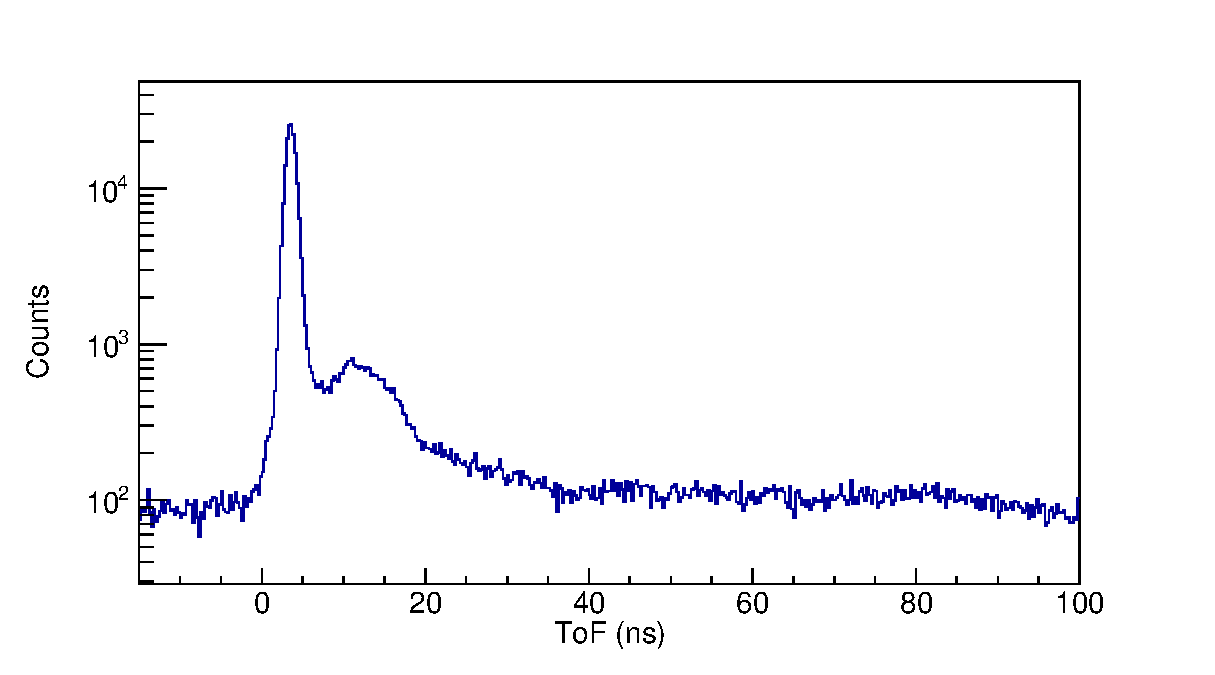
\includegraphics[width=0.80\textwidth]{example_gflash.eps}
	\caption{Gamma flash of measurement number 3, in semi-logarithmic scale.}
	\label{example_gflash}
\end{figure}

\subsection{Measurements} 
The time-of-flight measurements carried out to study the \Aliso \an reaction took place on April 17th and 18th.
The details of the dates, beam energies, flight path distances and accumulated beam (charge) on target of each experiment are listed in Table \ref{pulsed_measurements_table}.

\begin{table}[H]	%Tabla con datos de las medidas de haz pulsado
\centering
\begin{tabular}[c]{>{\bfseries}r||c|c|c|c}
	N& Energy (\unit{\keV}) & Distance (\unit{\cm}) & Charge (\unit{\micro\coulomb}) & Date\tablefootnote{All took place in 2023} \\ \hline	%TBD?incertidumbre en distancia?
	1&\num{5500}&\num{100.0(25)}&?? &April 17\textsuperscript{th}\\ \hline
	2&\num{5500}&\num{100.0(25)}&?? &April 18\textsuperscript{th}\\ \hline
	3&\num{7000}&\num{100.0(25)}&?? &April 18\textsuperscript{th}\\ \hline
	4&\num{8250}&\num{100.0(25)}&?? &April 18\textsuperscript{th}\\ \hline
	5&\num{8250}&\num{200.0(25)}&?? &April 18\textsuperscript{th}\\ \hline
\end{tabular}
\caption{Summary of the time-of-flight experiments carried out.}
\label{pulsed_measurements_table}
\end{table}

The single measurement on the 17th was a test and had a very low current, featuring also the highest tail in its $\gamma$-flash (\qty{30}{\percent} of counts), thus it was discarded in the analysis.
On the other hand, the experiments with the maximum beam energy was repeated at two different distances, in order to assess the expected improvement in neutron energy resolution.

\begin{figure}[H]
	\centering
	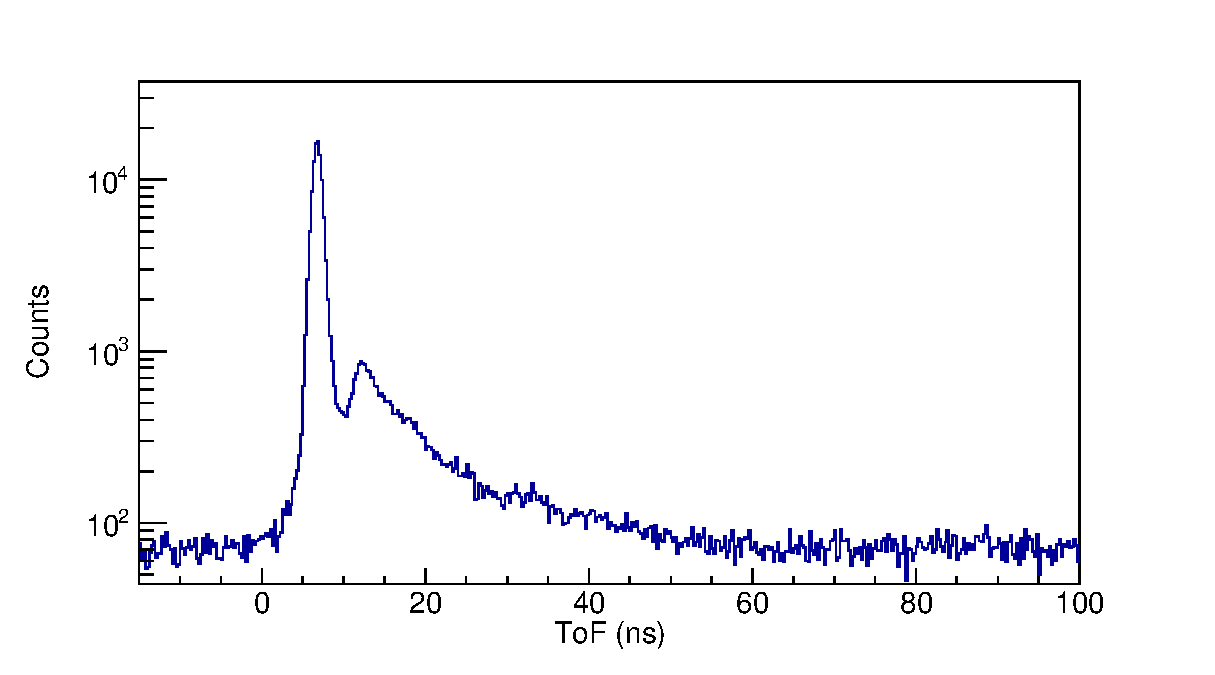
\includegraphics[width=0.80\textwidth]{uneven_gflash.eps}
	\caption{Particularly uneven gamma flash, corresponding to measurement 5.
	The bump after the first peak reaches \qty{10}{\percent} of the height.
	The tail is also long and clearly visible.}
	\label{uneven_gflash}
\end{figure}

\section{Data analysis}
The objective of our analysis is to obtain the energy spectra of the neutrons generated by the \an reactions.
To that end, we must first separate the gammas from the neutrons by using PSD, creating a Figure such as \ref{example_psd}.
We thus get the gamma flash and the neutron response for each measurement.

\begin{figure}[H]
	\centering
	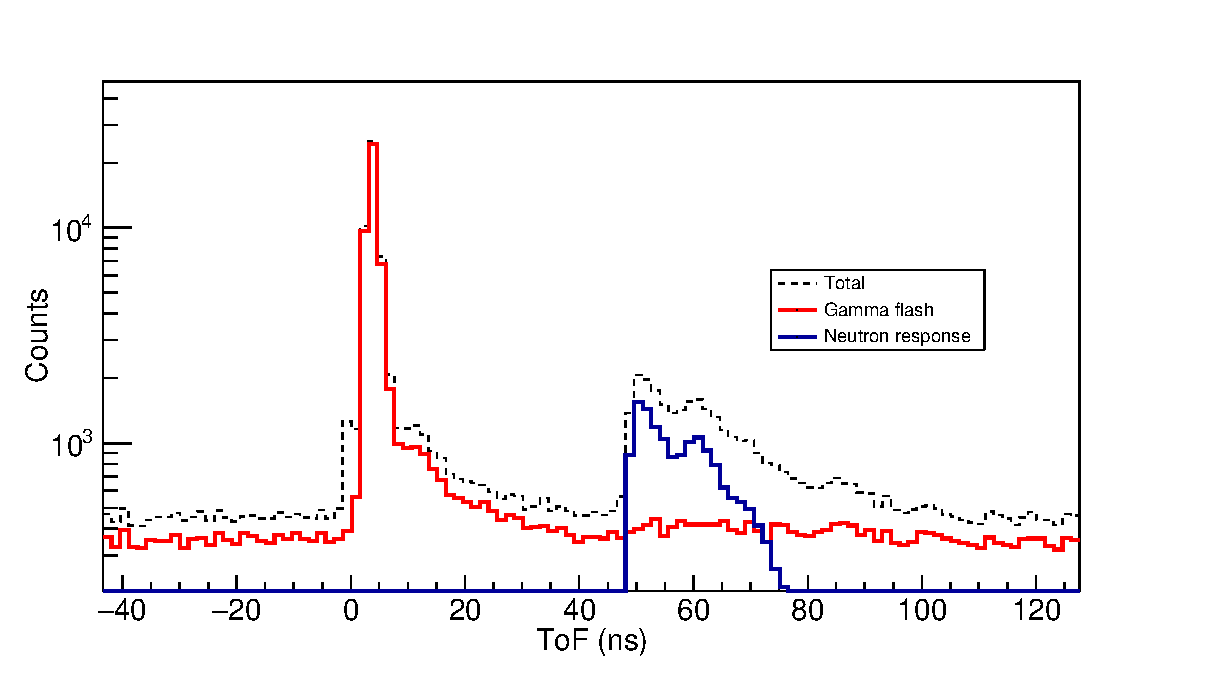
\includegraphics[width=0.80\textwidth]{separated_tof.eps}
	\caption{Gamma flash (blue) and neutron response (red), along with all counts (black) measurement number 2.}
	\label{separated_tof}
\end{figure}

To get the neutron energy spectra, we use two different methods of analysing the resulting histograms for each measurement.

\subsection{Simple method}
This method makes use mostly of the neutron response counts.
We use the gamma flash histogram exclusively to get its center, by taking as the centroid when fitting it to a gaussian.
We then calculate the ToF of each neutron as:
\begin{equation}
	\text{ToF} = t_n-t_\text{flash}+\frac{L}{c}
\end{equation}
with $t_n$ the timestamp (with respect to the signal from the chopper) of the neutron, $t_\text{flash}$ the center of the gamma flash, and $L/c$ the time it takes the gammas to get to the detector, i.e., the ToF of the gamma flash.
From each time-of-flight, we can then get the energy of the neutron as:
\begin{equation}
	E=\frac{1}{2} m_\text{n} \left( \frac{d}{\text{ToF}} \right)^2
\end{equation}
with $m_\text{n}$ the mass of the neutron.

Representing the calculated energy of every count in the neutron response in a histogram, we get the energy spectrum of the detected neutrons.
We correct it by dividing every bin by the detector's efficiency in energy (given by Figure \ref{monster_efficiency}).

To get the result per steradian, we divide by the number of steradians covered by the detector:
\[ \frac{\pi \cdot \text{detector radius}^2}{\cancel{4 \pi} \cdot \text{distance to target}^2}\cdot \cancel{4\pi}\unit{sr}  \]
We further correct it by dividing by the number of $\alpha$ particles (which we get from the current integrator) and the width of the bins.
The resulting plot (Figure \ref{pulsed_energysimple}) is the energy spectrum of the neutrons produced in the \an reactions.

\begin{figure}[H]
	\centering
	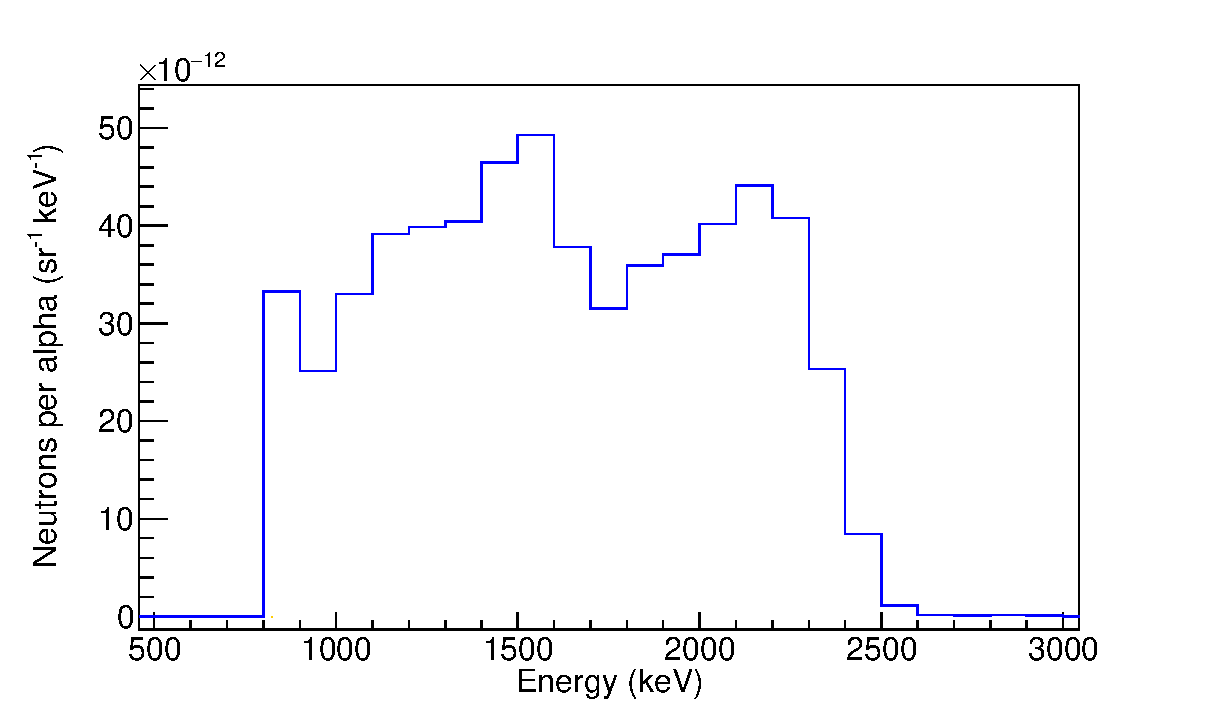
\includegraphics[width=0.80\textwidth]{pulsed_energysimple.eps}
	\caption{Resulting energy spectrum for measurement number 2 using the simple method.}
	\label{pulsed_energysimple}
\end{figure}

This method doesn't consider the shape of the alpha pulse, rather it assumes all of the neutrons are created at the same time, $d/c$ time before the center of the gamma flash.
This means that neutrons of the same energy generated by $\alpha$ particles arriving later will be interpreted as having lower energies, and viceversa.

Also, an excess of neutrons with very long ToF, that are deflected off the walls and take a longer path, will be detected.
This will create an excess of detections of low energy neutrons.
For the results (like Figure \ref{pulsed_energysimple}), we simply remove all counts for which efficiency would be under \qty{15}{\percent}.
A better solution would be to carry out the experiments with a shadow cone, which would absorb neutrons coming from directions other than the target's and allow us to study lower energies.

\subsection{Deconvolution}
We can take the shape of the alpha pulse into account by doing a deconvolution.
This is interesting, as it potentially solves some of the probles caused by the shape of the alpha pulse in the \textit{simple method}.
In order to do so, we fit the neutron response ToF histogram to a function that takes the gamma flash histogram as an input.

We use the gamma flash because, as previously noted, its shape will be the same as that of the alpha pulse, simply scaled by a certain factor and displaced $+L/c$ in the time axis.
This is because, every time an $\alpha$ particle hits the target, it will generate $K_\alpha$ gamma rays, a constant.
\\

The function that does the deconvolution holds \num{50} parameters to be adjusted by the fitting, each associated with a certain time-of-flight.
Their values correspond to the number of neutrons of a certain ToF produced per gamma ray detected in the gamma flash.

Their units are equivalent to 'number of neutrons per $\alpha$', but we don't know $K_\alpha$ to convert from gammas to $\alpha$ particles.
If we multiply the parameters by the total number of counts in the gamma flash, and divide by the number of incident $\alpha$ particles, they get units of neutrons per incident $\alpha$
\begin{equation}
	\frac{\text{detected neutrons}}{\text{detected gammas}}\cdot \frac{\text{detected gammas}}{\text{incident $\alpha$ particles}} = \frac{\text{detected neutrons}}{\text{incident $\alpha$ particles}}
\end{equation}
Doing it this way, we don't need to calculate $K_\alpha$, which would involve finding the efficiency of the detector for gammas in order to get the total number of gammas emmited.
After multiplying by that factor, the parameters are independent of the efficiency of the detector to $\gamma$-rays.
\\

Together, they form the neutron energy spectrum of the reaction, but in time-of-flight.
That is, the neutron response that would be generated by a single $\alpha$ particle.

If we multiply them by the total number of $\alpha$ particles and plot each parameter at their corresponding ToF, we get Figure \ref{pulsed_deconvolution_delta}, the neutron response that would be generated by a perfectly narrow alpha pulse.
The result is to remove the effect of the width and assymetry of the gamma flash.
We can see that the peaks become higher and more well defined; and the tail, lower.
This is because some of the neutrons detected later are actually faster, but just produced later by the tail of the alpha pulse.
The effect is that they are moved to lower ToFs.

Looking at it the other way around, we could say that the effect of the alpha pulse being wide is that the response to a Dirac delta pulse gets stretched horizontally.
\\

\begin{figure}[H]
	\centering
	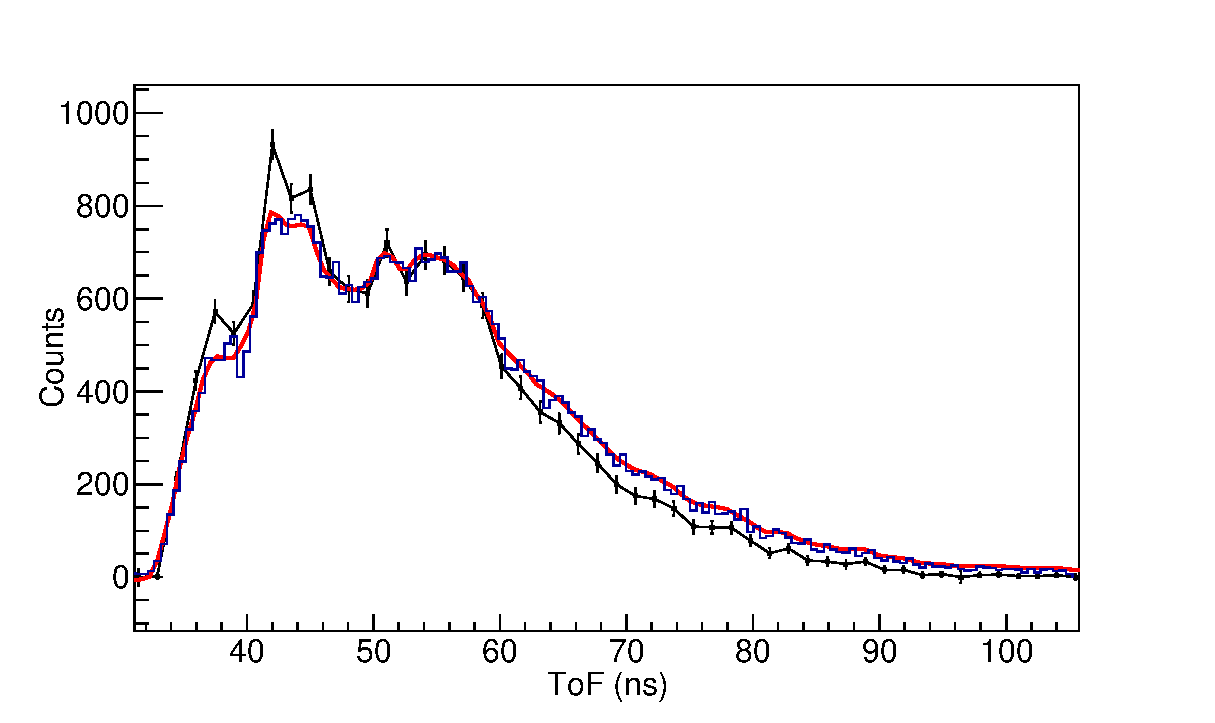
\includegraphics[width=0.80\textwidth]{pulsed_deconvolution_delta.eps}
	\caption{Measured neutron response histogram (blue), result of the fitted deconvolution function (red) and response to a Dirac delta pulse (black) for measurement number 4.}
	\label{pulsed_deconvolution_delta}
\end{figure}

In order to actually get the values of the parameters, we first need to fit the function to the experimental data.

The function is implemented as a C++ functor and the fitting is done by ROOT's \textit{fit} method.
In order for ROOT to be able to adjust the parameters, the function needs to output the neutron response for a given set of 50 parameters, so that it can compare the result to the measured neutron response histogram.

To that end, the function goes through every bin in the gamma flash histogram, which stands in for the alpha pulse.
It multiplies every parameter by the value of the bin, obtaining for each a number of neutrons produced at a different ToF.
It adds together the contribution of all bins, and the result is, if the parameters are right, the measured neutron response.

In order to determine the parameters, ROOT: runs the function, compares the result with the measurements, adjusts the parameters, then repeats; until a solution is found.
\\

This is computationally slow, as it needs to run through that loop many times.
The time it takes grows considerably with the number of parameters, and more than 50 was not considered viable.

In order to get better results when converting from ToF to energy, the parameters are equally spaced in between a minimum and a maximum in the energy space.
This means the parameters are more densely packed for high ToFs and more spaced for lower ToFs.
Because of that, when converting the parameters from ToF to energy, the distances between them in ToF need to be calculated for each, and taken into account.
\\

Converted from ToF to energy, the parameters will form the energy spectra of neutrons generated by a Dirac delta alpha pulse.
Once corrected by the efficiency of the detector using Figure \ref{monster_efficiency}, we get Figure \ref{pulsed_deconvolution}.
As with the \textit{simple method}, we have removed all counts for which MONSTER's efficiency would be under \qty{15}{\percent}.
The problem of scattered neutrons is inherent to the measurements and not due to the alpha pulse shape, so the deconvolution does nothing to alleviate it.

\begin{figure}[H]
	\centering
	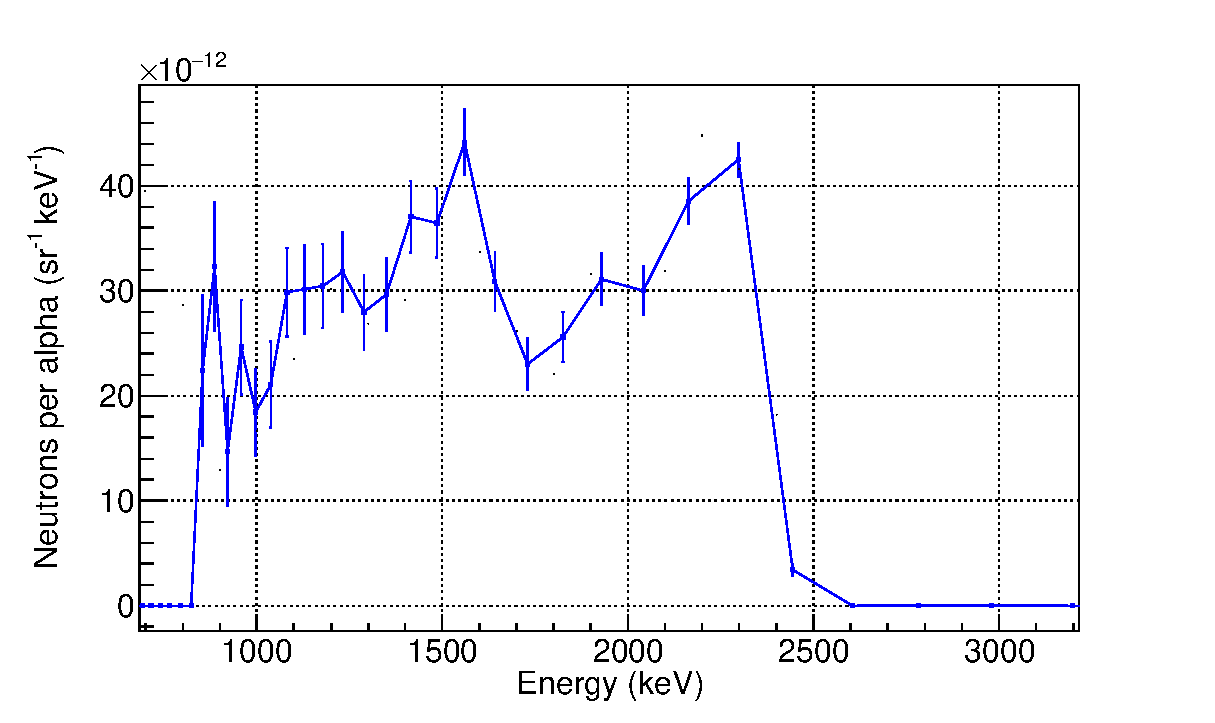
\includegraphics[width=0.80\textwidth]{pulsed_deconvolution.eps}
	\caption{Parameters resulting from the deconvolution, forming the energy spectrum for measurement number 2.}
	\label{pulsed_deconvolution}
\end{figure}

Figure \ref{pulsed_deconvolution} is the equivalent of \ref{pulsed_energysimple}, with the effects caused by the shape of the alpha pulse removed.
Both are plotted together in Figure \ref{pulsed_5mev}.

\section{Results}
Both the simple method and the deconvolution agree with each other quite well for all measurements, with expected differences:
\begin{itemize}
	\item The deconvolution effectively moves some of the lower energy counts in the simple method spectra to higher energies, as they were created in the tail of the alpha pulses.
		Because of this, the deconvolution spectra are lower than the simple method's for low energies, and higher for higher energies.
	\item The deconvolution seems to only sometimes achieve better definition, which can be seen in the sharper peaks in the spectra.
		This is could in theory be improved with more parameters, but we run into problems with computing time and overfitting to noise.
\end{itemize}

Data to compare to only exists for the \qty{5.5}{\MeV} thick target yield spectrum, in the G. J. H. Jacobs and H. Liskien paper \cite{jacobs}.
We can see that the deconvolution matches quite well, while the simple method overestimates it, specially for low energies (Figure \ref{pulsed_5mev}).
This is expected, because of the simple method taking neutrons with longer trajectories as having lower energies.

\begin{figure}[H]
	\centering
	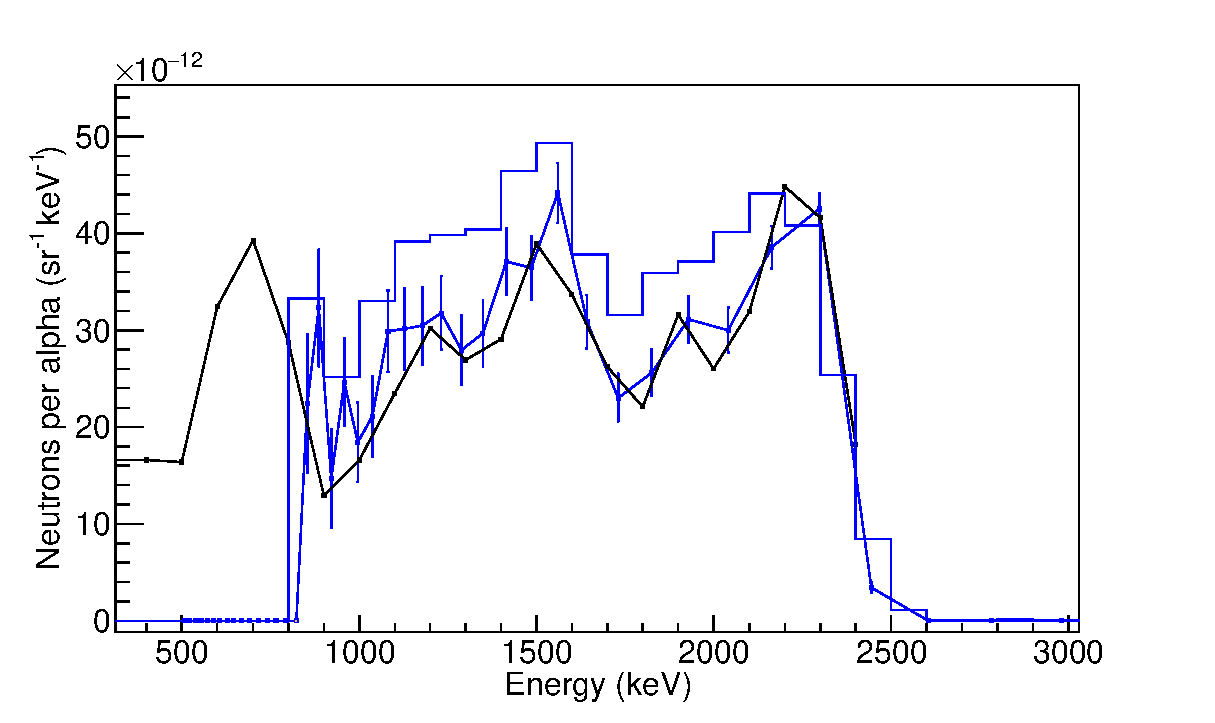
\includegraphics[width=0.80\textwidth]{pulsed_5mev.eps}
	\caption{Neutron spectra for \qty{5500}{\keV}.
	G. J. H. Jacobs and H. Liskien data (black), simple method (blue histogram) and deconvolution (blue squares).}
	\label{pulsed_5mev}
\end{figure}

The error bars shown for the deconvolution are those automatically calculated by ROOT when doing the fitting.
Calculating the uncertainty of a deconvolution method is complicated, and the good agreement with the literature shows that it is an improvement over the simple method.
The fact that the error bars mostly cover the literature data indicates that they are a reasonable enough estimate of uncertainty for showing where the true values might be at higher energies (where we have no data to compare to).
\\

Because of the high amount of noise, we are ignoring all neutrons for which the detector's efficiency would be under \qty{15}{\percent}.
This means that we cannot see the structure under \qty{1000}{\keV} reported by the literature.
In order to study the low energy part of neutron spectra at CNA, we would require a shadow cone, or some other means of removing scattered neutrons.
\\

For higher \an energies, there is no data to compare to.
However, we can calculate the maximum possible energy for neutrons, given the Q of the reaction and the cinematics.
We can see (Figure \ref{pulsed_results}) that that energy is surpassed in all cases, by several hundreds of \unit{\keV}.
This is probably because of the limited resolution of the detector.

We can compare both measurements at \qty{8.5}{\MeV} and see that, for lower energies, the higher distance seems to have improved the resolution: the peak at around \qty{1800}{\keV} is higher and narrower.
For the energy limt, it does not seem to have had any effect whatsoever.
However, there are no points to compare after the limit: the first parameter goes to 0 in both cases.
Thus, there could be an improvement and we wouldn't see it.

Comparing their \textit{simple method} histograms, the measurement at higher energies is consistently higher, probably due to a higher percentage of the counts being noise.
\\

\begin{figure}[H]
	\centering
	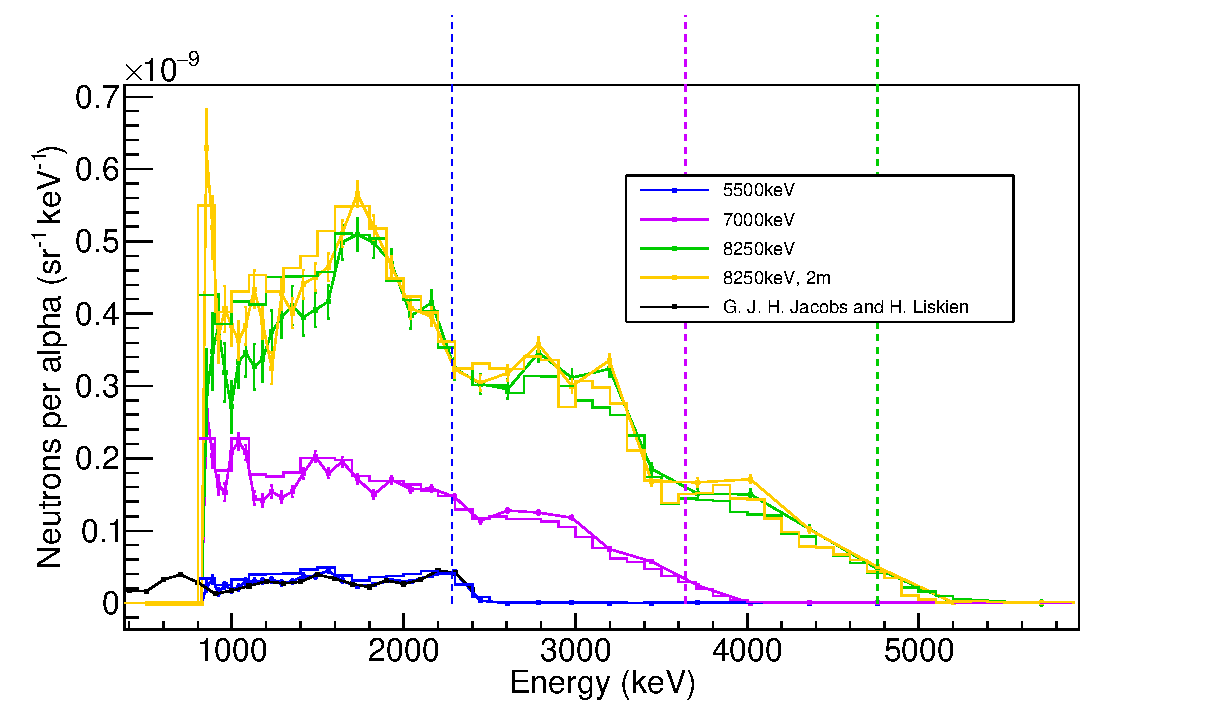
\includegraphics[width=0.80\textwidth]{pulsed_results.eps}
	\caption{G. J. H. Jacobs and H. Liskien data (black) and results for all of the time-of-flight measurements.
	The histograms are the simple method, the connected squares are the results of deconvolution, and the vertical dotted lines are the theoretical maximum neutron energies.}
	\label{pulsed_results}
\end{figure}

The sudden increase of cross section near the lower energy cutoff for all measurements is probably not due to a structure in the neutron spectra, but to an excess of scattered neutrons that.
Raising the cutoff further would remove them, but deprive us of a large part of the spectra.
\\

In summary, the deconvolution succeeds in moving low energy counts created by the tail of the alpha pulses to high energies, but only somewhat seems to improve the energy definition of the experiment.
The low energy part of the spectra cannot be seen due to noise, but it could be reduced with a shadow cone or other such system.
Where we can compare, the deconvolution measurements agree well with the literature, while the \textit{simple method} ones overestimate.

\chapter{Conclusions}
\section{Thick target yield}
For the \Aliso\an thick target yield activation measurements, results from the two analysis methods employed agree within \qty{1}{\percent}, meaning we can stick with the more standard \textit{decay} method.
Detectors agree with eachother within \qty{8}{\percent} for April and within \qty{4}{\percent} for February, with one detector (LaBr\textsubscript{3}(1) and LaBr\textsubscript{3}(2), respectively) being consistently higher than the other.
This tells us there is a systematic error when dealing with multiple detectors, that changes when repeating measurements.

When comparing measurements of the same energy in different months the agreement is good, within around \qty{3}{\percent}, which tells us the results are consistent with each other.
The comparison with the literature, however, shows a large disagreement, with our results being higher by a factor of \num{1.90(9)}, a systematic error.
Because the shape shown by our data matches the one of the literature, the error must be a multiplicative factor, and most likely an error in the data analysis that remains undiscovered.

To solve this problem, the data analysis must either be checked for errors in the code (again) or redone from scratch.
If the error still cannot be found, repeating the measurements could be warranted.
\\

\section{Neutron energy spectra}
For the \Aliso\an neutron energy spectra measurements through time-of-flight, the deconvolution results show good agreement with the previous measurement in the literature, and an improvement over the more straightforward, \textit{simple method}.
However, such data to compare to exists only for the lowest \an energy measured, \qty{5.5}{\MeV}.

The deconvolution succeeds in correcting for the long tail and other assymetries in the $\alpha$ pulses created by the accelerator, but doesn't improve the energy resolution much.
Increasing the distance of the MONSTER detector from 1 to \qty{2}{\m} also does not improve resolution by a lot, and is probably not worth the decreased statistics.
\\

Due to the large background of scattered neutrons, the low energy part of the spectra (under approximately \qty{1000}{\keV}) has a large excess of counts and cannot be properly measured.
A clear improvement would be to do following measurements with a shadow cone, able to absorb scattered neutrons coming from directions other than the target's.

\section{Viability of \an measurements at CNA/HiSPANoS}
The results show that measurement of \an reactions are viable with the CNA accelerator.
Activation measurements are in good agreement with each other, and if the systematic error can be found, could be done at more energies and for other materials without any changes to the procedure or equipment.

For time-of-flight measurements, a shadow cone or other system for eliminating scattered neutrons is necessary in order to be able to measure the lower energy parts of spectra.
As for the assymetry of the pulses, results could be improved with either a more sofisticated deconvolution system or by adapting the accelerator to better support $\alpha$ particles.
However, the setup is able to give reasonable measurements as-is by using a very simple deconvolution process.



\begin{thebibliography}{5}
	\bibitem{jacobs}G. J. H. Jacobs and H. Liskien, Energy Spectra of Neutrons produced by $\alpha$ particles in thick targets of light elements, Annals of Nuclear Energy 10, 541 (1983), \url{https://doi.org/10.1016/0306-4549(83)90003-8}
	\bibitem{hispanos}B Fernández et al 2020 J. Phys.: Conf. Ser. 1643 012033, HiSPANoS facility and the new neutron beam line for TOF measurements at the Spanish National Accelerator Lab (CNA), \url{https://doi.org/10.1088/1742-6596/1643/1/012033}
	\bibitem{guerrero2008}C. Guerrero et al., Analysis of the BC501A neutron detector signals using the true pulse shape, Nuclear Instruments and Methods in Physics Research A 597 (2008) 212–218, \url{https://doi.org/10.1016/j.nima.2008.09.017}
	\bibitem{astro1}F. Käppeler et al., Rev. Mod. Phys. 83, 157 – 193 (2011), The \textit{s} process: Nuclear physics, stellar models, and observations, \url{https://doi.org/10.1103/RevModPhys.83.157}
	\bibitem{astro2}J. Pereira and F. Montes, Phys. Rev. C 93, 034611 (2016), Theoretical uncertainty of \an reactions relevant for the nucleosynthesis of light r-process nuclei in neutrino-driven winds, \url{https://doi.org/10.1103/PhysRevC.93.034611}
	\bibitem{neutron_in_an}NV.A. Kudryavtsev, P. Zakhary. B. Easeman, Neutron production in \an reactions, Nucl. Instrum. Methods Phys. Res. A 972 (2020), \url{https://doi.org/10.1016/j.nima.2020.164095}
	\bibitem{MANY}N. Mont-Geli et al., miniBELEN: A modular neutron counter for \an reactions, EPJ Web of Conf., 284 (2023) 06004, \url{https://doi.org/10.1051/epjconf/202328406004}
%	\bibitem{}\url{https://doi.org/10.1016/j.nima.2009.04.032}
	\bibitem{nucleardatasheets}M. Shamsuzzoha Basunia, Nuclear Data Sheets 111, 2331 (2010)
	\bibitem{INDC}S. S. Westerdale et al., Technical Report, INDC(NDS)-0836 (2022), \url{https://www-nds.iaea.org/publications/indc/indc-nds-0836.pdf}
	\bibitem{CNA}Gómez-Camacho, J., García López, J., Guerrero, C. et al., Research facilities and highlights at the Centro Nacional de Aceleradores (CNA). Eur. Phys. J. Plus 136, 273 (2021), \url{https://doi.org/10.1140/epjp/s13360-021-01253-x}
	\bibitem{labr}Alain Iltis et al., Lanthanum halide scintillators: Properties and applications, Nuclear Instruments and Methods in Physics Research Section A: Accelerators, Spectrometers, Detectors and Associated Equipment, Volume 563, Issue 2 (2006), \url{https://doi.org/10.1016/j.nima.2006.02.192.}
	\bibitem{MONSTER}A R Garcia et al., MONSTER: a time of flight spectrometer for $\beta$-delayed neutron emission measurements, 2012 JINST 7 C05012, \url{http://dx.doi.org/10.1088/1748-0221/7/05/C05012}
	\bibitem{ej301}NEUTRON/GAMMA PSD EJ-301, EJ-309, \url{https://eljentechnology.com/products/liquid-scintillators/ej-301-ej-309}
	\bibitem{jacobssupport1}R. Heaton et al., Nuclear Instruments and Methods A 276, 529 (1989)
	\bibitem{jacobssupport2}J. K. Bair and J. Gomez del Campo, Neutron Yields from Alpha-Particle Bombardment, Nuclear Science and Engineering 71, 18 (1979), \url{https://doi.org/10.13182/NSE71-18}
	\bibitem{CAEN}CAEN 751 Waveform Digitizer Family, CAEN SpA, \url{https://www.caen.it/subfamilies/751-digitizer-family/}
	\bibitem{ROOT}Rene Brun and Fons Rademakers, ROOT - An Object Oriented Data Analysis Framework, Proceedings AIHENP'96 Workshop, Lausanne, Sep. 1996, Nucl. Inst. \& Meth. in Phys. Res. A 389 (1997) 81-86. See also "ROOT" [software], Release 6.28/04, \url{https://doi.org/10.5281/zenodo.848818}
\end{thebibliography}

\end{document}
